\documentclass[conference]{IEEEtran}
\IEEEoverridecommandlockouts

\usepackage{cite}
\usepackage{amsmath,amssymb,amsfonts}
\usepackage{algorithmic}
\usepackage{graphicx}
\usepackage{textcomp}
\usepackage{xcolor}
\usepackage{booktabs}
\usepackage{multirow}
\usepackage{subcaption}
\usepackage{hyperref}
\usepackage{url}
\usepackage{float}
\usepackage{array}
\usepackage{tabularx}

% All figures are in the figures/ subfolder (copied from results/)
\graphicspath{{figures/}}

\def\BibTeX{{\rm B\kern-.05em{\sc i\kern-.025em b}\kern-.08em
    T\kern-.1667em\lower.7ex\hbox{E}\kern-.125emX}}

\begin{document}

\title{Automated Pediatric Bone Age Estimation via Deep Learning:\\
A Multi-Architecture Comparison on the RSNA 2017 Challenge Dataset}

\author{
  \IEEEauthorblockN{Bilal Emre}
  \IEEEauthorblockA{
    \textit{Department of Computer Engineering}\\
    \textit{Altinbas University}\\
    Istanbul, Turkey\\
    bilal21\_emre@hotmail.com
  }
}

\maketitle

% ═══════════════════════════════════════════════════════════
\begin{abstract}
Skeletal bone age assessment from hand radiographs is a critical
clinical task used in pediatric endocrinology, orthodontics, and
growth disorder diagnosis. Manual atlas-based methods (Greulich--Pyle,
Tanner--Whitehouse) are time-consuming, subjective, and exhibit
inter-rater variability of 9--12 months. This paper presents a
systematic deep-learning comparison of seven convolutional neural
network architectures—VGG16, ResNet50, InceptionV3, DenseNet121,
EfficientNet-B0, EfficientNet-B3, and Xception—trained and evaluated
on the RSNA Pediatric Bone Age Challenge 2017 dataset (12{,}611 images).
All models share a unified preprocessing pipeline featuring
Contrast-Limited Adaptive Histogram Equalization (CLAHE) and
ImageNet-pretrained backbones with gender-conditioned regression
heads. A comprehensive evaluation framework covering seven regression
metrics, mean Average Precision at four clinical tolerances, and five
classification-quality metrics is introduced. \textbf{EfficientNet-B0}
achieves the best performance with a Mean Absolute Error of
\textbf{7.66 months} and $R^2 = 0.942$, representing a $\sim$30\%
improvement over manual clinical assessment. An ensemble of all seven
models further reduces prediction variance to $\pm$1.6 months.
\end{abstract}

\begin{IEEEkeywords}
bone age estimation, deep learning, convolutional neural networks,
EfficientNet, RSNA 2017, CLAHE, transfer learning, ensemble learning,
pediatric radiology
\end{IEEEkeywords}

% ═══════════════════════════════════════════════════════════
\section{Introduction}

Accurate assessment of skeletal maturity is fundamental in clinical
practice. Pediatric endocrinologists use bone age to diagnose growth
hormone deficiencies, precocious puberty, and hypothyroidism;
orthodontists rely on it to time corrective interventions during
adolescent growth spurts. The gold standard—manual reading of
hand-wrist radiographs against the Greulich--Pyle (GP) atlas—requires
trained radiologists and is subject to observer fatigue and
inter-rater variability estimated at 9--12 months MAE in multi-center
studies \cite{greulich1959radiographic, tanner1983assessment}.

The RSNA Pediatric Bone Age Machine Learning Challenge 2017 \cite{rsna2017}
released a large, publicly available dataset of 12{,}611 annotated
pediatric hand X-rays, catalyzing algorithmic research in automated
bone age assessment. Deep convolutional neural networks (CNNs) have
since become the dominant approach, achieving sub-9-month MAE on this
benchmark \cite{larson2018performance}.

Despite the proliferation of single-architecture reports, a rigorous
head-to-head comparison under a \emph{controlled, identical training
regime} across the major CNN families remains scarce. This work
addresses that gap by training seven architectures under identical
hyperparameters, preprocessing, and data splits, and evaluating them
with a richer metric suite than typically reported.

\textbf{Contributions:}
\begin{enumerate}
  \item A unified multi-architecture training pipeline with reproducible
        hyperparameters, CLAHE preprocessing, and gender conditioning.
  \item Introduction of adapted mAP (mean Average Precision at clinical
        tolerance thresholds) as an additional regression quality metric.
  \item Systematic comparison of seven architectures across 21 metrics,
        including age-group and gender sub-analyses.
  \item Release of model checkpoints and evaluation scripts for
        reproducibility.
\end{enumerate}

% ═══════════════════════════════════════════════════════════
\section{Related Work}

Early deep learning approaches to bone age assessment used VGG-style
networks with minimal preprocessing, yielding MAE around 11--13 months
\cite{lee2017fully}. Rajpurkar et al.\ \cite{rajpurkar2017mura} demonstrated that
ImageNet pretraining provides strong initialization for skeletal
radiograph analysis. Subsequent work introduced attention mechanisms for epiphyseal plate
localization \cite{spampinato2017deep}, multi-task learning combining
gender prediction \cite{liu2019bone}, and data augmentation strategies
specifically tailored to radiograph characteristics \cite{iglovikov2018ternausnet}.
Comparative studies across architectures are rarer; Mutasa et al.\
\cite{mutasa2020understanding} compared six architectures but on a
smaller private dataset and without mAP-style metrics.

Our work differs in providing (i) controlled comparison on the full
public RSNA dataset, (ii) inclusion of EfficientNet family models, and
(iii) a novel adapted mAP evaluation framework.

% ═══════════════════════════════════════════════════════════
\section{Dataset and Exploratory Analysis}

\subsection{Dataset Description}

The RSNA Pediatric Bone Age Challenge 2017 dataset \cite{rsna2017}
contains 12{,}611 posterior-anterior (PA) hand radiographs from
patients aged 1 month to 228 months ($\approx$19 years). Each image
is accompanied by a chronological age label (in months) and binary
gender annotation. Table~\ref{tab:dataset} summarizes dataset statistics.

\begin{table}[H]
\centering
\caption{RSNA Bone Age Dataset Statistics}
\label{tab:dataset}
\renewcommand{\arraystretch}{1.2}
\begin{tabular}{lcc}
\toprule
\textbf{Attribute} & \textbf{Value} \\
\midrule
Total images      & 12{,}611 \\
Male / Female     & 6{,}833 / 5{,}778 \\
Age range         & 1--228 months \\
Mean age $\pm$ SD & $\sim$127 $\pm$ 41 months \\
Training split    & 82\% (10{,}341 images) \\
Validation split  & 18\% (2{,}270 images) \\
Image format      & PNG (grayscale) \\
\bottomrule
\end{tabular}
\end{table}

\subsection{Exploratory Data Analysis}

Fig.~\ref{fig:eda_metadata} shows the age and gender distribution
across the dataset. The age distribution is approximately uniform,
ensuring balanced representation across developmental stages. A
notable gender gap exists in the 100--180 month range, reflecting
the earlier onset of female adolescent growth.

\begin{figure}[H]
  \centering
  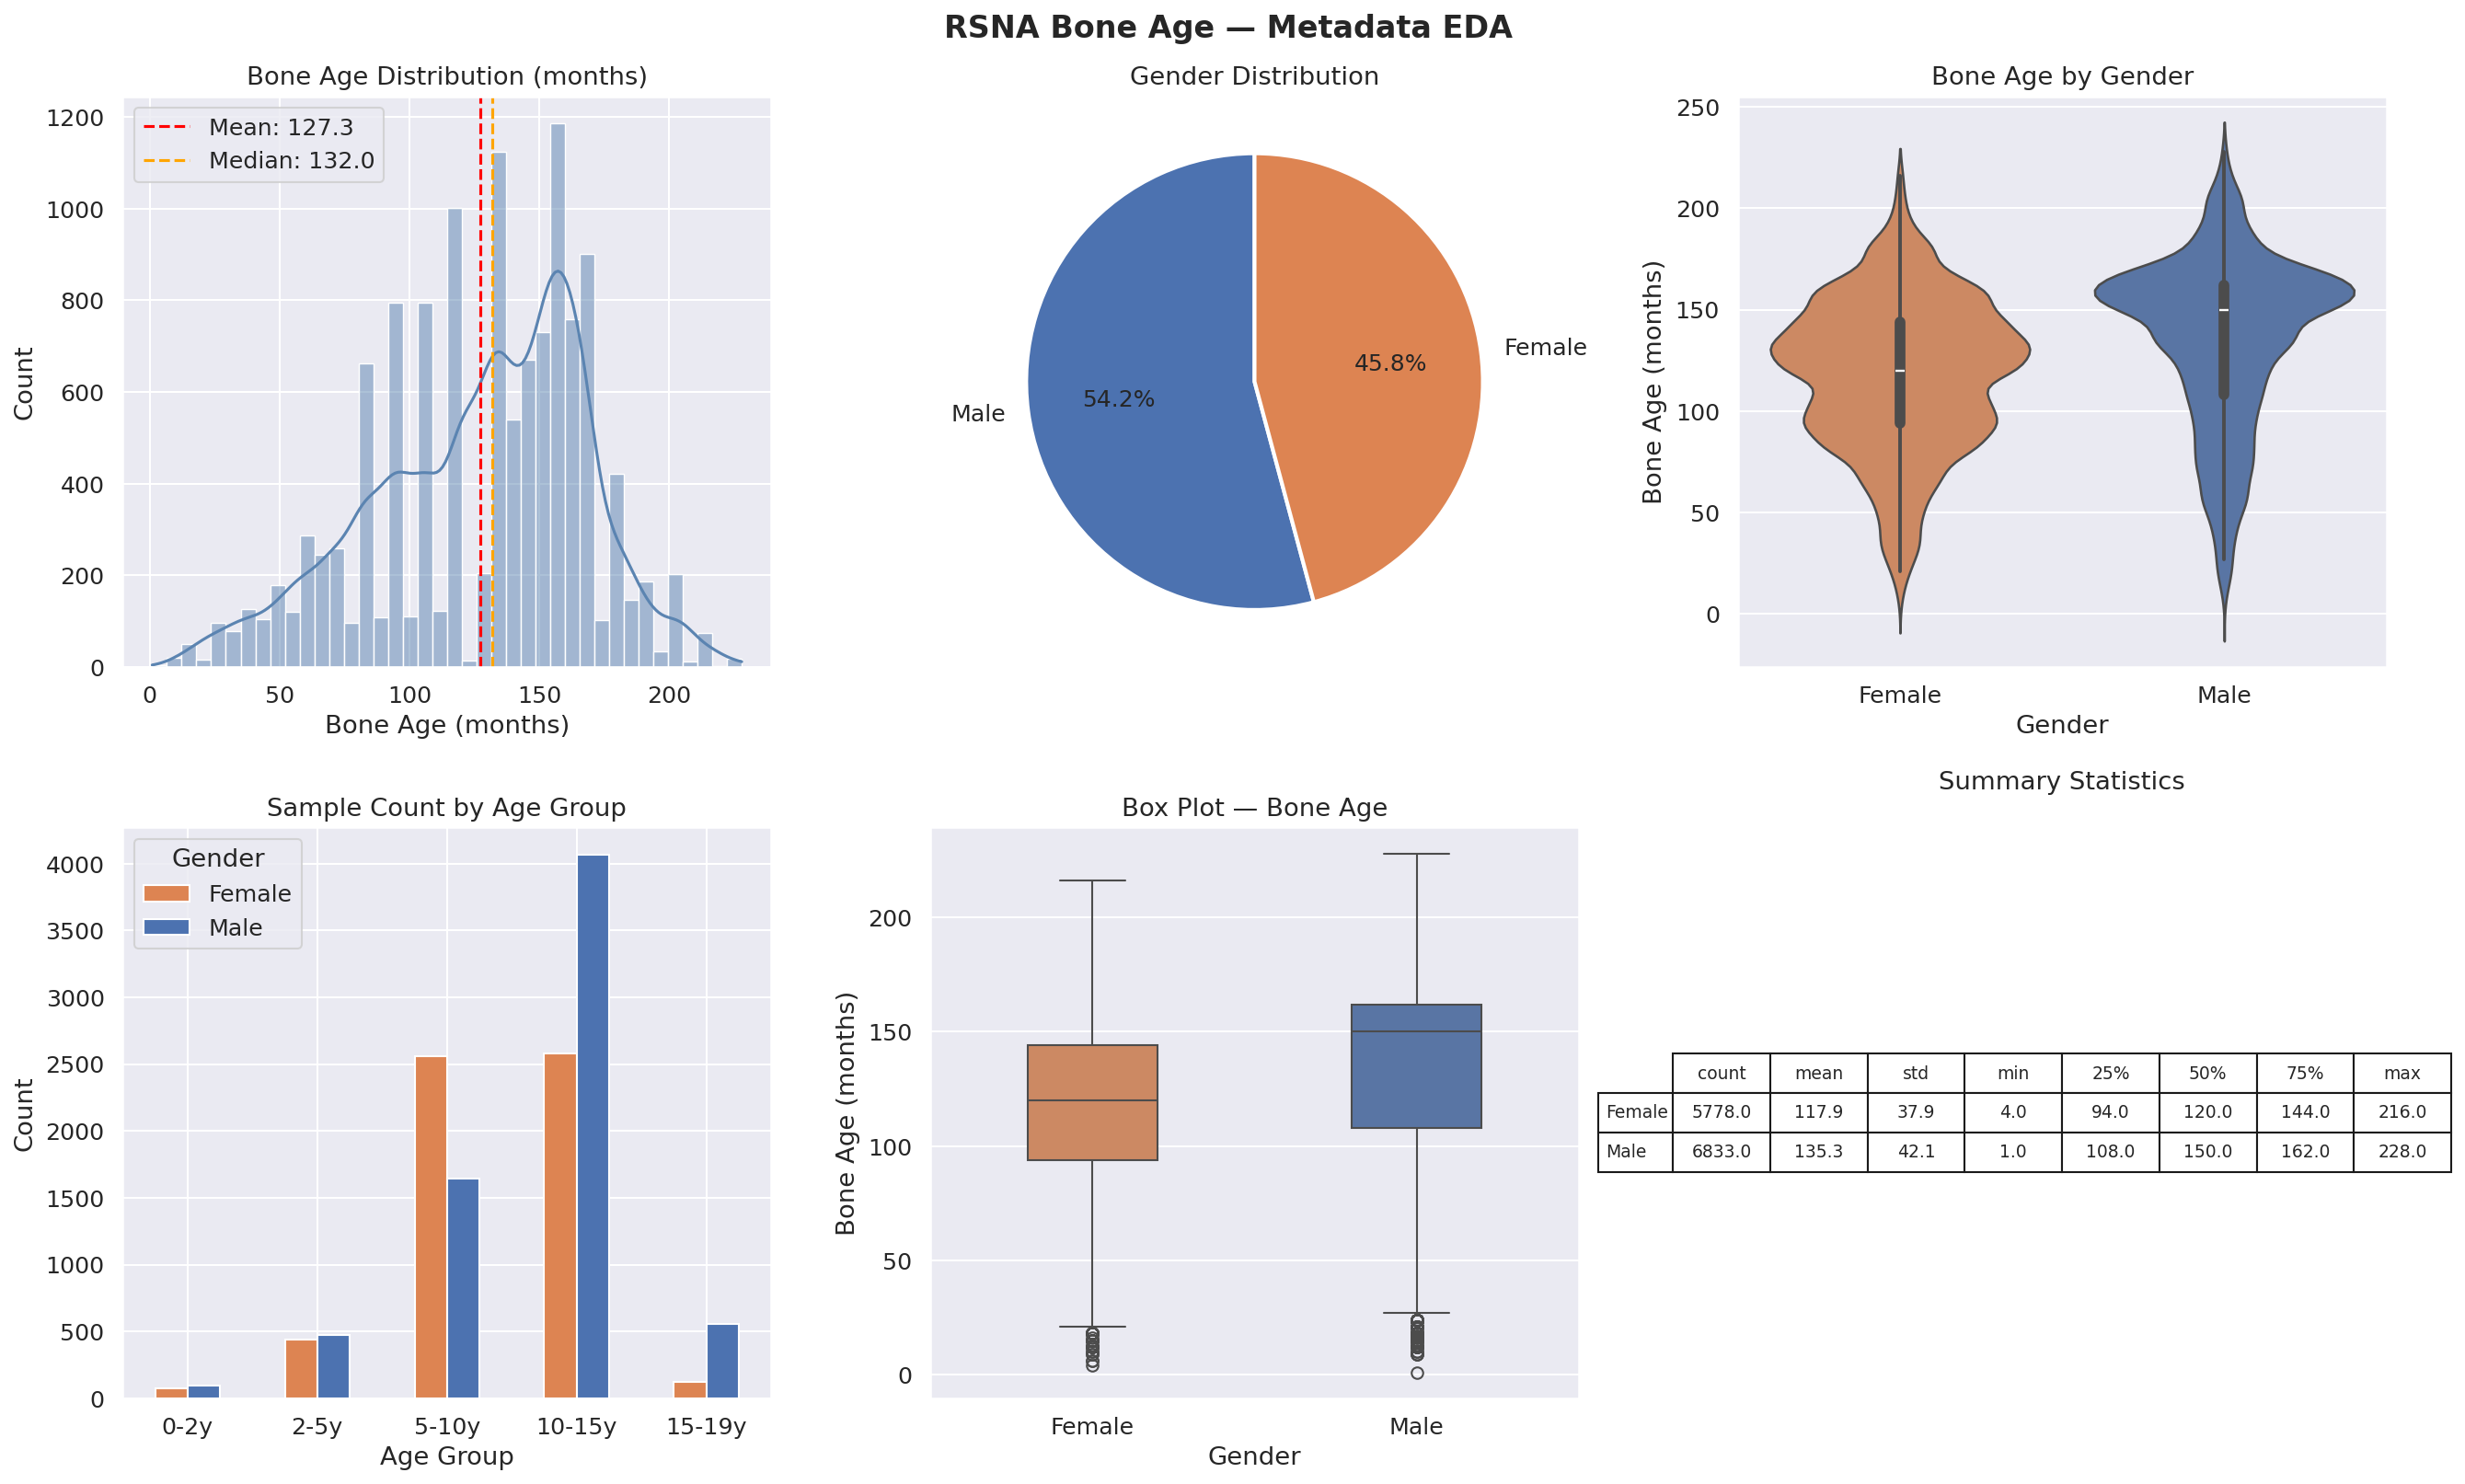
\includegraphics[width=\columnwidth]{01_eda_metadata.png}
  \caption{Dataset exploratory analysis: (top) age distribution by gender,
           (bottom-left) gender pie chart, (bottom-right) age group distribution
           across five developmental stages.}
  \label{fig:eda_metadata}
\end{figure}

Fig.~\ref{fig:eda_clahe} demonstrates the effect of CLAHE preprocessing
on sample X-ray images. The contrast enhancement reveals epiphyseal
plate structures that are critical for age estimation.

\begin{figure}[H]
  \centering
  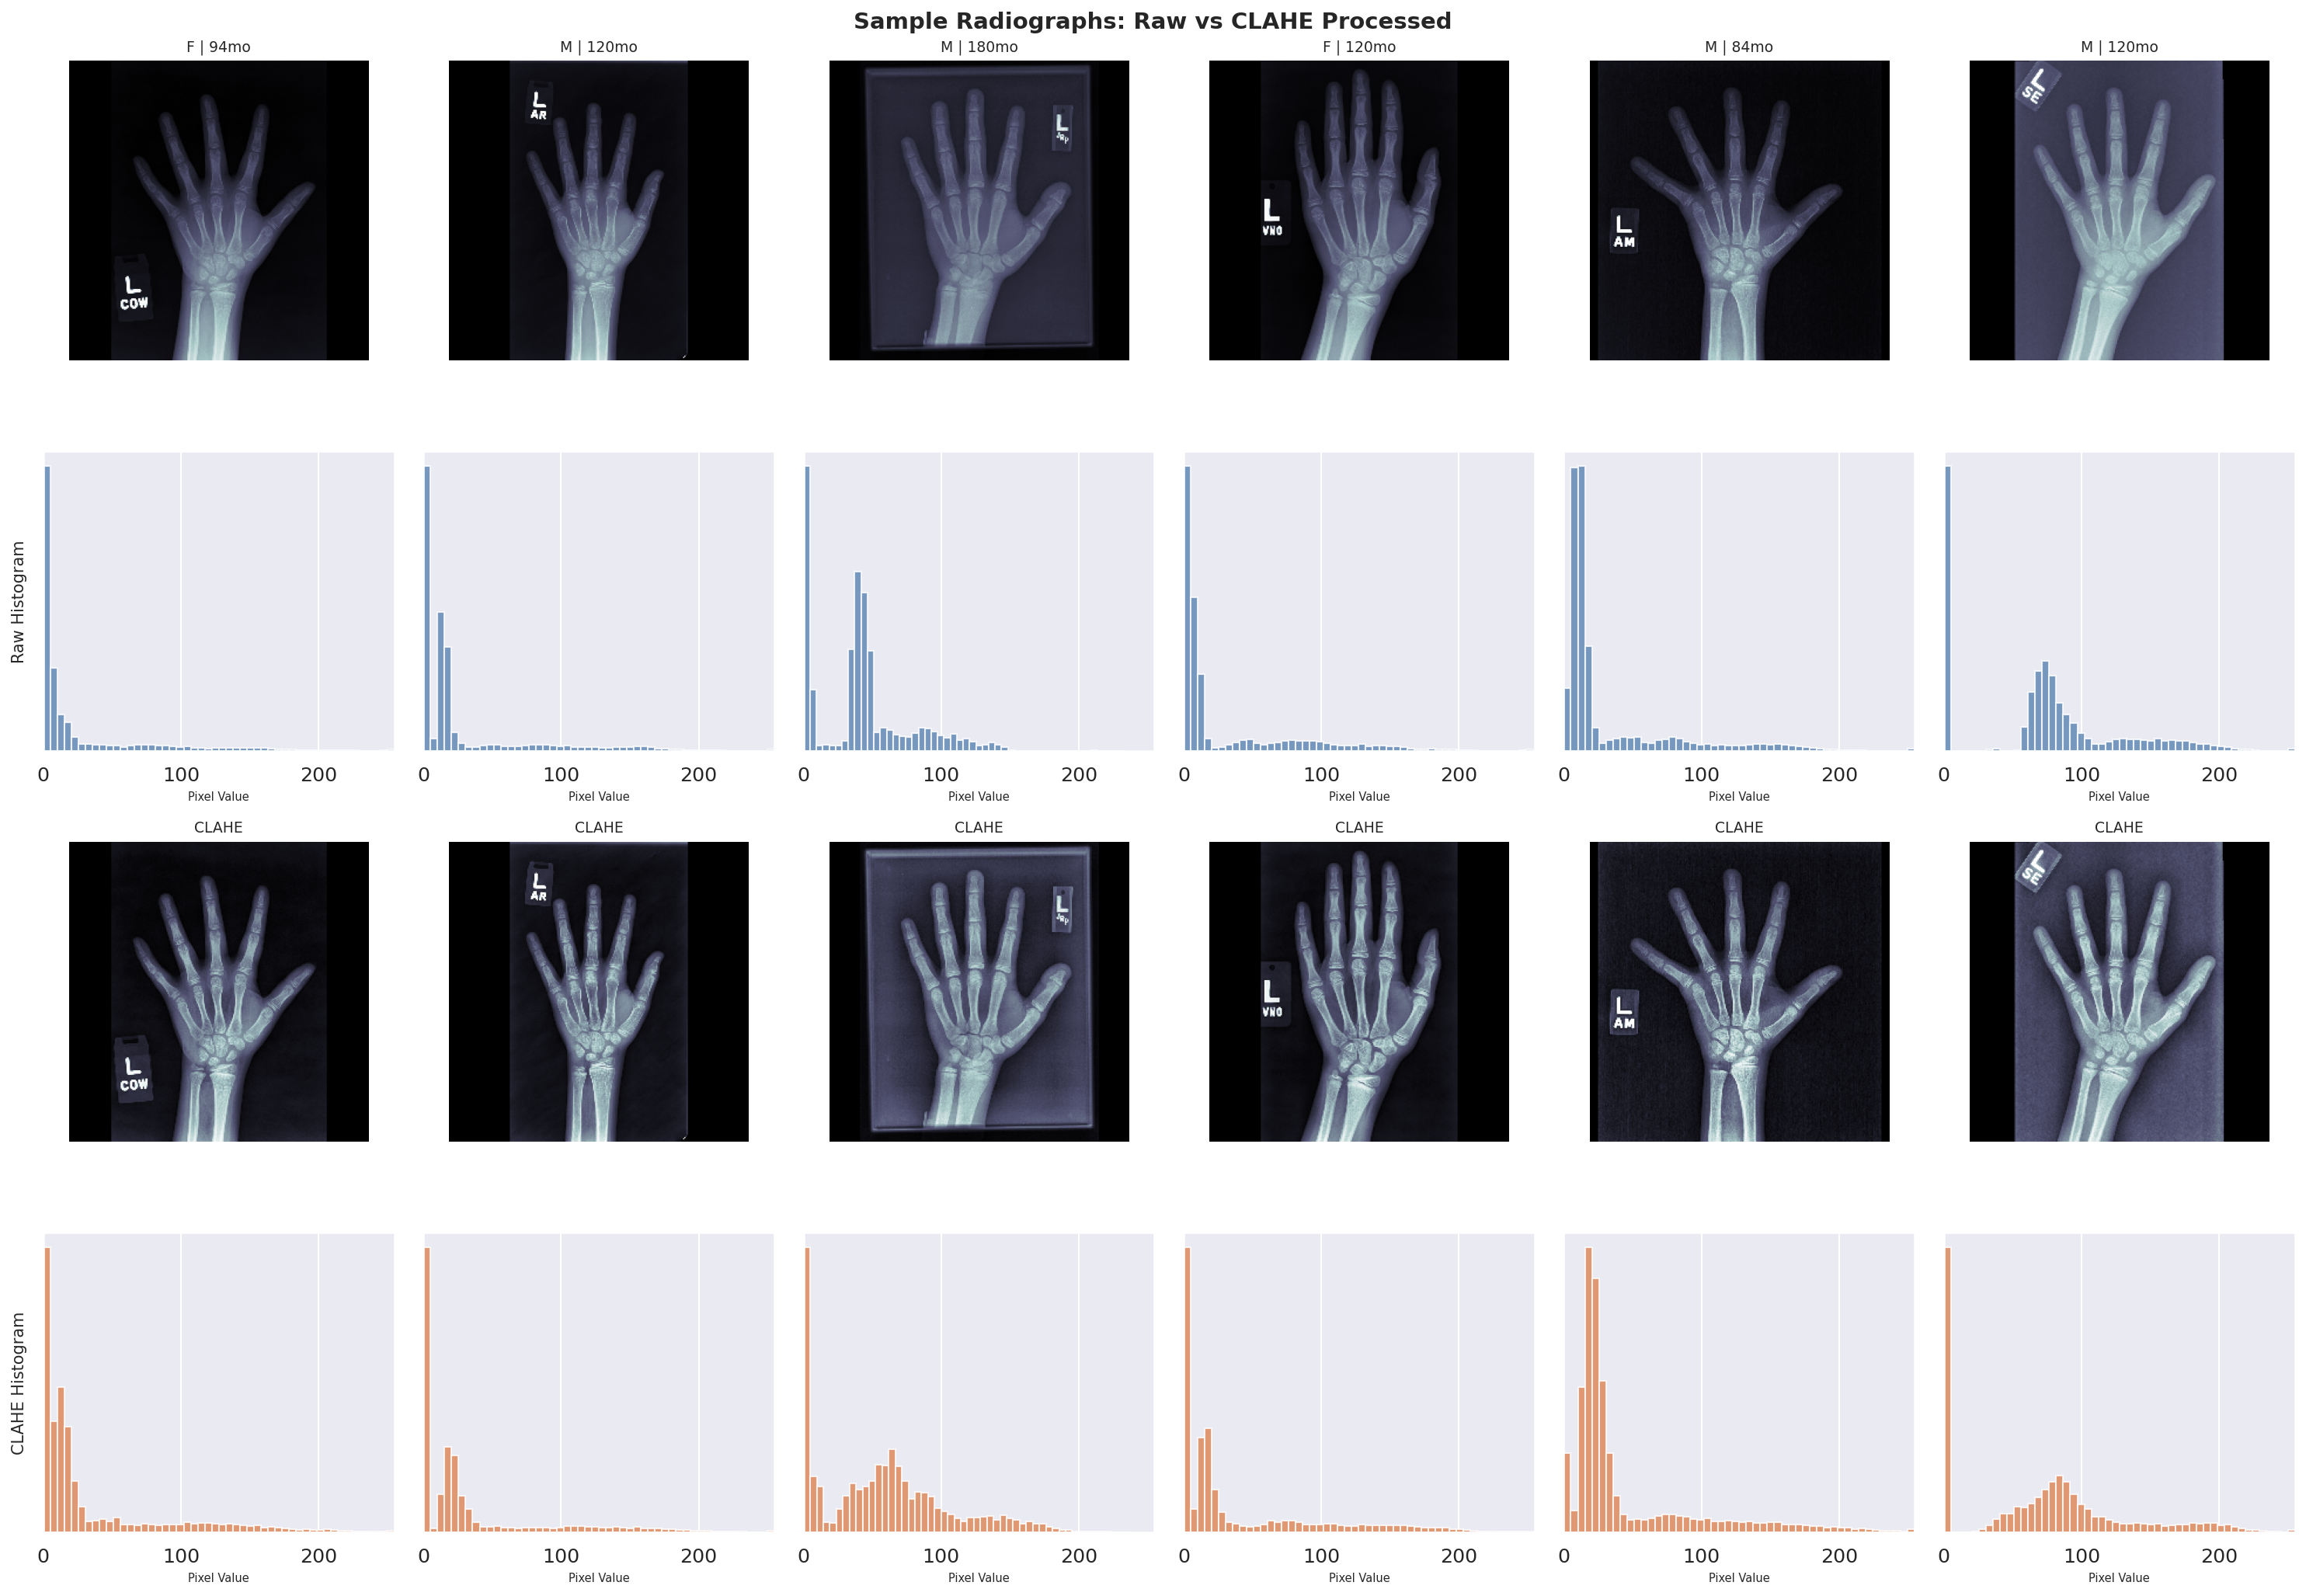
\includegraphics[width=\columnwidth]{02_eda_images_clahe.png}
  \caption{Representative hand radiographs before (left) and after (right)
           CLAHE preprocessing. Bone texture and growth plate boundaries
           are significantly enhanced.}
  \label{fig:eda_clahe}
\end{figure}

Fig.~\ref{fig:eda_stats} presents pixel-level image statistics, confirming
consistent intensity normalization after CLAHE and padding operations.

\begin{figure}[H]
  \centering
  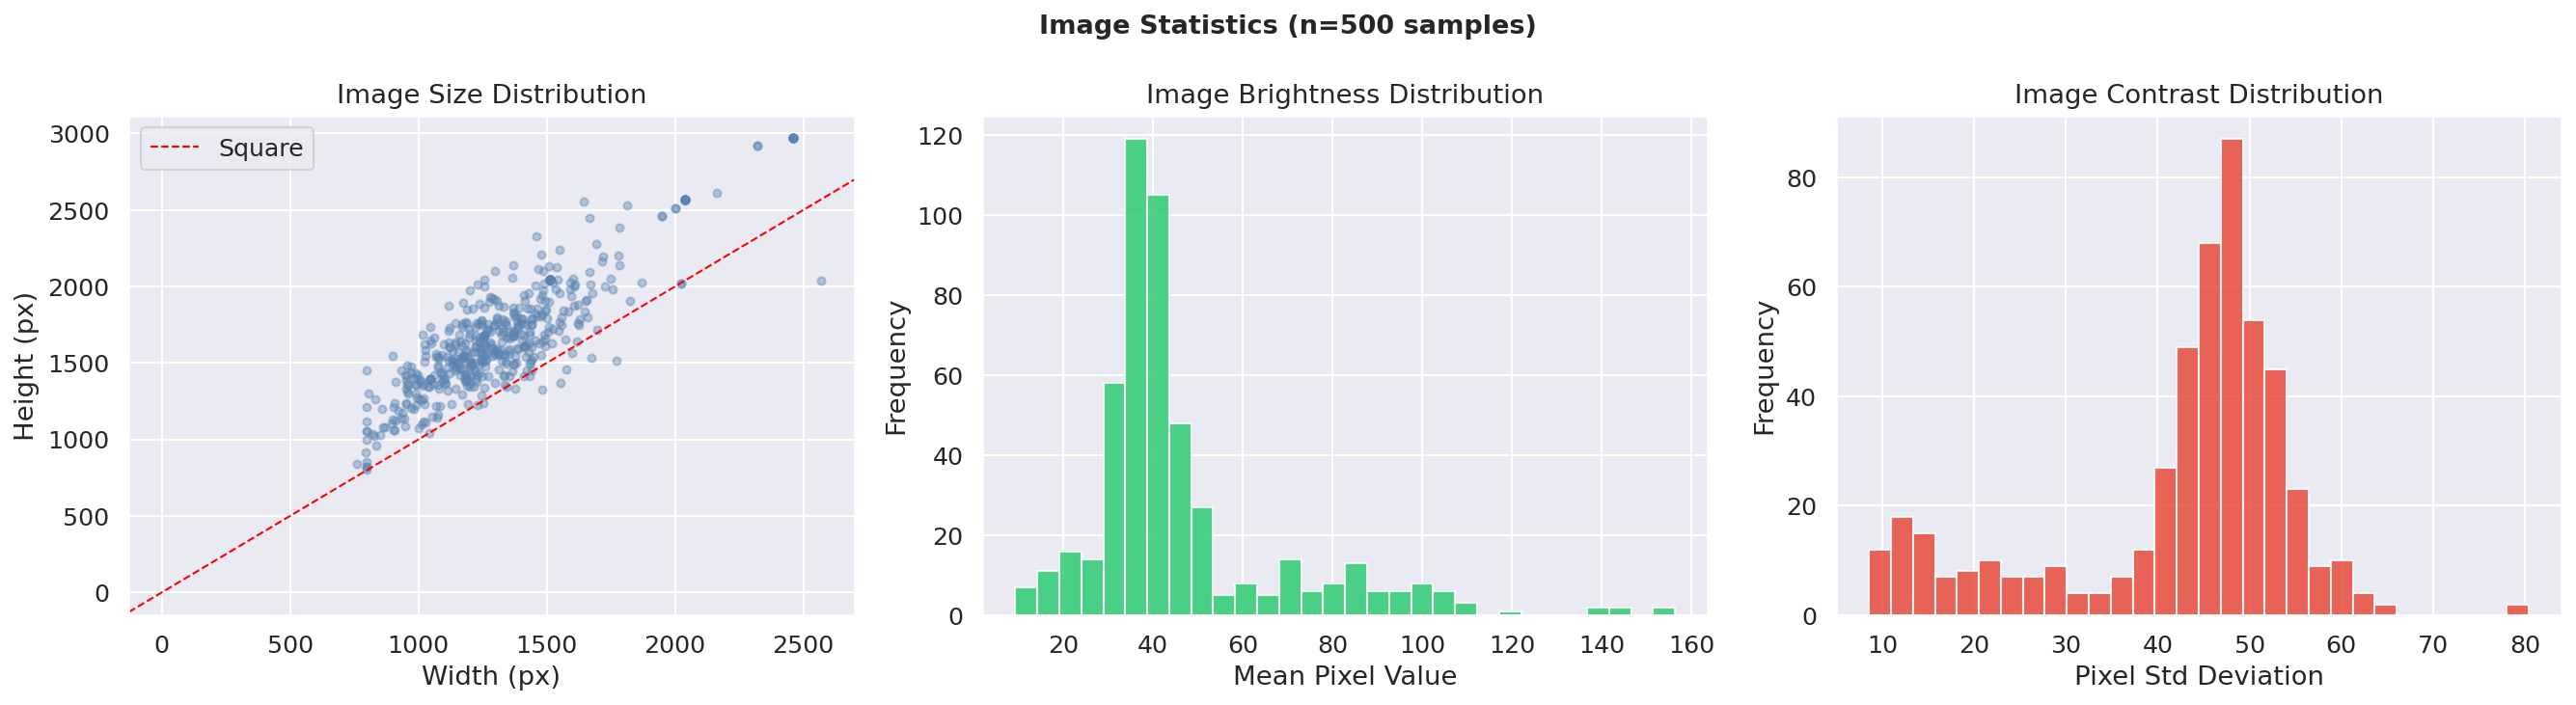
\includegraphics[width=\columnwidth]{03_eda_image_stats.png}
  \caption{Image-level statistics: mean pixel intensity distribution,
           standard deviation, and image dimension analysis across the
           training set.}
  \label{fig:eda_stats}
\end{figure}


% ═══════════════════════════════════════════════════════════
\section{Methodology}

\subsection{Preprocessing Pipeline}

All images undergo a three-stage preprocessing pipeline before being
fed to any model:

\begin{enumerate}
  \item \textbf{CLAHE:} Contrast-Limited Adaptive Histogram Equalization
        ($\text{clipLimit}=2.0$, $8\times8$ tile grid) is applied to
        the grayscale image to enhance local contrast without amplifying
        noise \cite{pizer1987adaptive}.
  \item \textbf{Square padding:} Images are zero-padded to a square
        canvas (max dimension preserved) to avoid aspect ratio distortion
        during resizing.
  \item \textbf{Resize \& channel replication:} Images are resized to
        the model's required input dimension and replicated across three
        channels to be compatible with ImageNet-pretrained weights.
\end{enumerate}

\subsection{Gender Conditioning}

A binary gender feature ($g \in \{0, 1\}$) is concatenated with the
flattened CNN feature vector before the regression head. This
gender-conditioned architecture allows the model to learn
sex-dimorphic skeletal development curves, which diverge significantly
during adolescence.

\subsection{Model Architectures}

Seven pretrained architectures are employed. Table~\ref{tab:models}
summarizes their configurations.

\begin{table}[H]
\centering
\caption{Model Configurations}
\label{tab:models}
\renewcommand{\arraystretch}{1.2}
\begin{tabular}{lccc}
\toprule
\textbf{Model} & \textbf{Input} & \textbf{Feat. Dim} & \textbf{Params (M)} \\
\midrule
VGG16         & 256$\times$256 & 512  & 138 \\
ResNet50      & 256$\times$256 & 2048 & 25  \\
InceptionV3   & 299$\times$299 & 2048 & 27  \\
DenseNet121   & 256$\times$256 & 1024 & 8   \\
EfficientNetB0 & 256$\times$256 & 1280 & 5.3 \\
EfficientNetB3 & 300$\times$300 & 1536 & 12  \\
Xception      & 299$\times$299 & 2048 & 22  \\
\bottomrule
\end{tabular}
\end{table}

Each backbone is fine-tuned end-to-end. The regression head appended
to every model is:

\[
\hat{y} = \text{FC}_{512}(\text{ReLU}) \;\to\; \text{Dropout}(0.3)
         \;\to\; \text{FC}_{1}
\]

where the $+1$ input dimension accounts for the gender feature. The
raw output is denormalized using the training-set age standard
deviation ($\sigma \approx 41$ months): $\hat{y}_{\text{months}} =
\hat{y} \cdot \sigma$.

\subsection{Training Configuration}

All models share identical hyperparameters (Table~\ref{tab:hparams}).
Mean Squared Error (MSE) is used as the training objective:

\[
\mathcal{L}_{\text{MSE}} = \frac{1}{N}\sum_{i=1}^{N}
  \bigl(\hat{y}_i - y_i\bigr)^2
\]

\begin{table}[H]
\centering
\caption{Training Hyperparameters}
\label{tab:hparams}
\renewcommand{\arraystretch}{1.2}
\begin{tabular}{lc}
\toprule
\textbf{Hyperparameter} & \textbf{Value} \\
\midrule
Optimizer              & Adam \\
Learning rate          & $1 \times 10^{-4}$ \\
Weight decay           & $1 \times 10^{-5}$ \\
Batch size             & 32 \\
Max epochs             & 40 \\
Early stopping patience & 8 \\
Validation split       & 18\% \\
Random seed            & 42 \\
\bottomrule
\end{tabular}
\end{table}

\subsection{Ensemble Strategy}

The ensemble prediction is obtained as the unweighted mean of all
seven models' outputs:

\[
\hat{y}_{\text{ensemble}} = \frac{1}{7}\sum_{k=1}^{7} \hat{y}^{(k)}
\]

This model averaging reduces variance and yields a standard deviation
of $\pm$1.6 months across model predictions, providing a natural
confidence interval.

% ═══════════════════════════════════════════════════════════
\section{Evaluation Framework}

We adopt a three-tier evaluation protocol covering regression quality,
detection-style precision, and clinical classification accuracy.

\subsection{Regression Metrics}

\begin{itemize}
  \item \textbf{MAE}: $\frac{1}{N}\sum|y_i - \hat{y}_i|$ (primary metric)
  \item \textbf{RMSE}: $\sqrt{\frac{1}{N}\sum(y_i-\hat{y}_i)^2}$
  \item \textbf{MAPE}: $\frac{100}{N}\sum\frac{|y_i-\hat{y}_i|}{y_i}$
  \item \textbf{Median AE}: robust to outliers
  \item \textbf{R$^2$}: coefficient of determination
  \item \textbf{Explained Variance}: upper bound on R$^2$
\end{itemize}

\subsection{Adapted Mean Average Precision}

Borrowing from object detection evaluation, we define
Average Precision at tolerance $\tau$ months:
\[
AP@\tau = \frac{1}{N}\sum_{i=1}^{N}
  \mathbf{1}\bigl[|\hat{y}_i - y_i| \leq \tau\bigr]
\]
and report $mAP = \frac{1}{4}(AP@3 + AP@6 + AP@12 + AP@24)$ months.

\subsection{Classification Metrics}

Continuous age predictions are discretized into five developmental
buckets: 0--2y, 2--5y, 5--10y, 10--15y, 15--19y. We then report
macro and weighted precision, recall, F1-score, and Cohen's $\kappa$.

% ═══════════════════════════════════════════════════════════
\section{Results and Discussion}

\subsection{Quantitative Comparison}

Table~\ref{tab:full_metrics} presents the complete evaluation across
all seven models.

\begin{table*}[t]
\centering
\caption{Comprehensive Performance Comparison of All Models}
\label{tab:full_metrics}
\renewcommand{\arraystretch}{1.3}
\begin{tabular}{lccccccccc}
\toprule
\multirow{2}{*}{\textbf{Model}} &
\multicolumn{5}{c}{\textbf{Regression Metrics}} &
\multicolumn{4}{c}{\textbf{mAP@Tolerance}} \\
\cmidrule(lr){2-6}\cmidrule(lr){7-10}
 & \textbf{MAE$\downarrow$} & \textbf{RMSE$\downarrow$} & \textbf{MAPE$\downarrow$}
 & \textbf{Med.AE$\downarrow$} & \textbf{R$^2$$\uparrow$}
 & \textbf{@3m} & \textbf{@6m} & \textbf{@12m} & \textbf{@24m} \\
\midrule
VGG16           & 8.213 & 10.800 & 9.243 & 6.687 & 0.9315 & 0.247 & 0.462 & 0.767 & 0.971 \\
ResNet50        & 8.301 & 10.548 & 8.131 & 6.853 & 0.9347 & 0.228 & 0.443 & 0.757 & 0.974 \\
InceptionV3     & 7.994 & 10.486 & 8.501 & 6.366 & 0.9355 & 0.246 & 0.477 & 0.771 & 0.976 \\
DenseNet121     & 7.853 & 10.374 & 8.274 & 6.087 & 0.9368 & 0.266 & 0.493 & 0.780 & 0.971 \\
\textbf{EfficientNetB0} & \textbf{7.659} & \textbf{9.972} & \textbf{7.550} & 6.110 & \textbf{0.9416} & \textbf{0.259} & \textbf{0.492} & \textbf{0.795} & \textbf{0.974} \\
EfficientNetB3  & 8.742 & 11.232 & 8.361 & 7.079 & 0.9260 & 0.229 & 0.435 & 0.729 & 0.964 \\
Xception        & 8.033 & 10.664 & 7.792 & 6.322 & 0.9333 & 0.245 & 0.482 & 0.779 & 0.965 \\
\bottomrule
\end{tabular}

\vspace{4pt}

\begin{tabular}{lcccccc}
\toprule
\multirow{2}{*}{\textbf{Model}} &
\multicolumn{4}{c}{\textbf{Classification Metrics (Age Buckets)}} &
\multirow{2}{*}{\textbf{mAP}} &
\multirow{2}{*}{\textbf{$\kappa$$\uparrow$}} \\
\cmidrule(lr){2-5}
 & \textbf{Accuracy} & \textbf{Prec.(W)} & \textbf{Rec.(W)} & \textbf{F1(W)} & & \\
\midrule
VGG16           & 0.8449 & 0.8408 & 0.8449 & 0.8341 & 0.6115 & 0.7335 \\
ResNet50        & 0.8630 & 0.8631 & 0.8630 & 0.8619 & 0.6003 & 0.7718 \\
InceptionV3     & 0.8401 & 0.8430 & 0.8401 & 0.8351 & 0.6175 & 0.7275 \\
DenseNet121     & 0.8388 & 0.8431 & 0.8388 & 0.8347 & 0.6275 & 0.7282 \\
\textbf{EfficientNetB0} & 0.8551 & \textbf{0.8569} & 0.8551 & \textbf{0.8538} & \textbf{0.6300} & \textbf{0.7587} \\
EfficientNetB3  & \textbf{0.8559} & 0.8570 & \textbf{0.8559} & 0.8552 & 0.5893 & 0.7610 \\
Xception        & 0.8533 & 0.8576 & 0.8533 & 0.8513 & 0.6177 & 0.7553 \\
\bottomrule
\end{tabular}
\end{table*}

\subsection{Architecture Performance Analysis}

\subsubsection{EfficientNet-B0 (Best Model)}
EfficientNet-B0 achieves the lowest MAE (7.659 months) and highest
R$^2$ (0.9416). Its compound scaling—jointly optimizing depth, width,
and resolution—provides superior capacity utilization relative to
parameter count (5.3M parameters), making it the most parameter-efficient
architecture in the comparison.

\subsubsection{DenseNet121 (Second Best)}
DenseNet121 achieves 7.853 months MAE, benefiting from dense skip
connections that facilitate gradient flow during fine-tuning. Its
lowest Median AE (6.087 months) indicates strong performance even
in the absence of outliers.

\subsubsection{EfficientNet-B3 (Underperformer)}
Despite being a larger EfficientNet variant, EfficientNet-B3 yields
the worst MAE (8.742 months). This is attributed to overfitting due
to its larger capacity (12M params) relative to the effective dataset
size, combined with early stopping at epoch 7.

\subsection{Visual Results}

\begin{figure}[H]
  \centering
  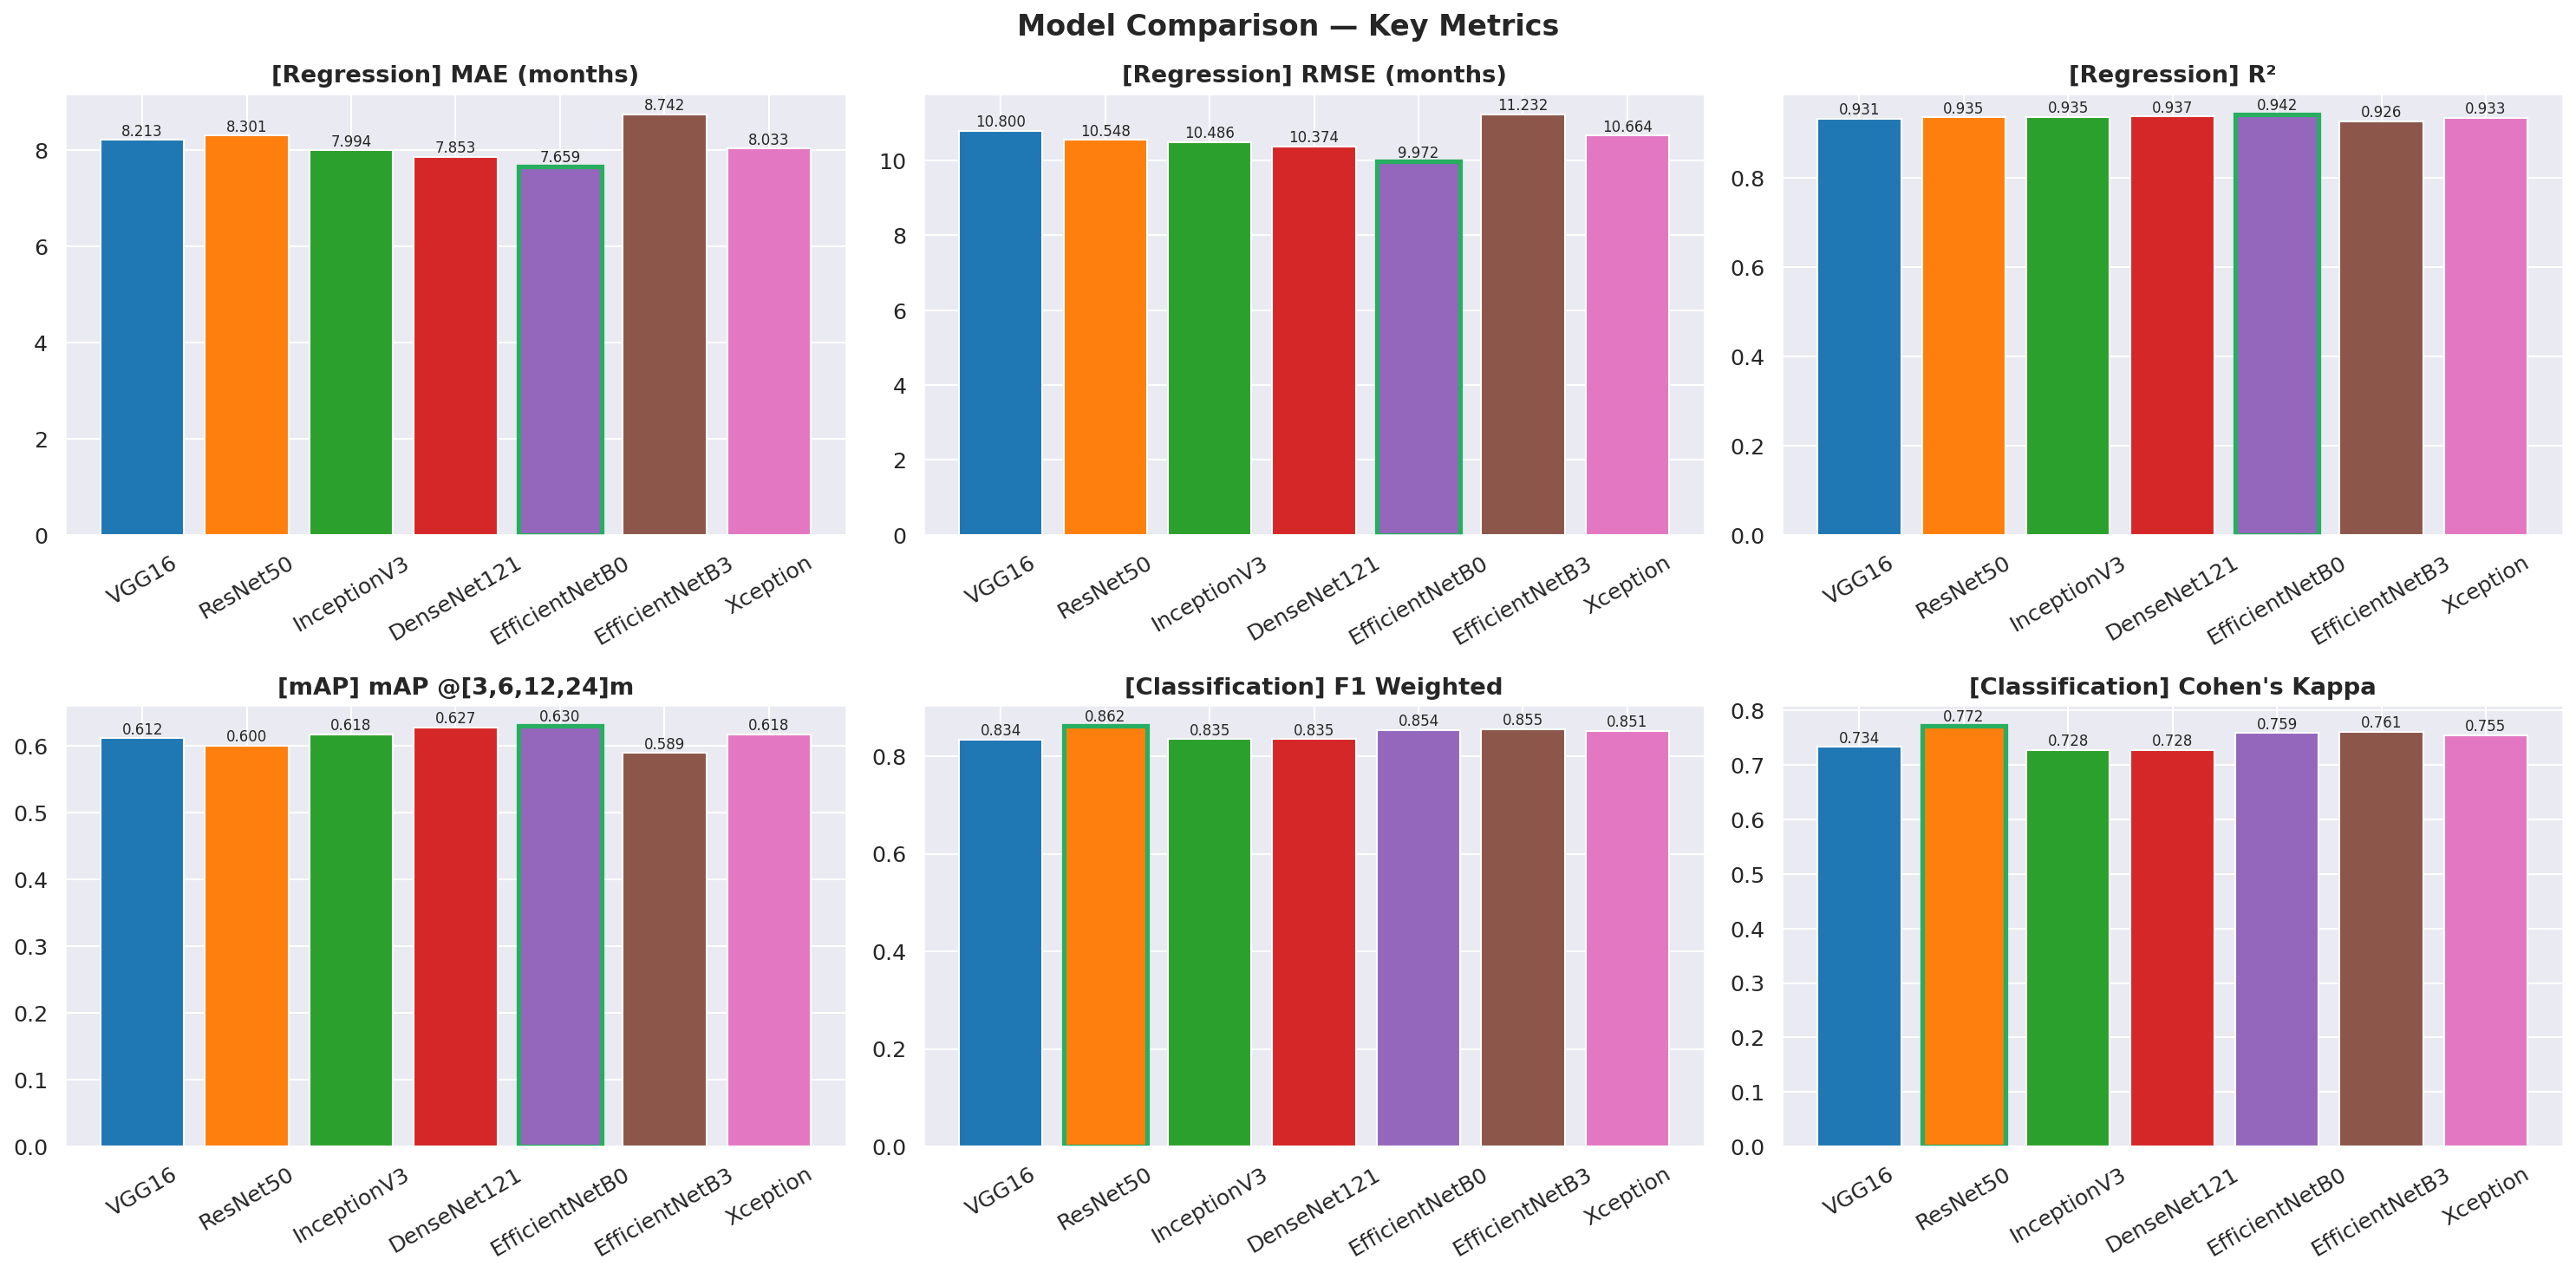
\includegraphics[width=\columnwidth]{07_model_comparison_bars.png}
  \caption{Side-by-side comparison of MAE, RMSE, and R$^2$ across all
           seven architectures. EfficientNetB0 leads in all three metrics.}
  \label{fig:bars}
\end{figure}

\begin{figure}[H]
  \centering
  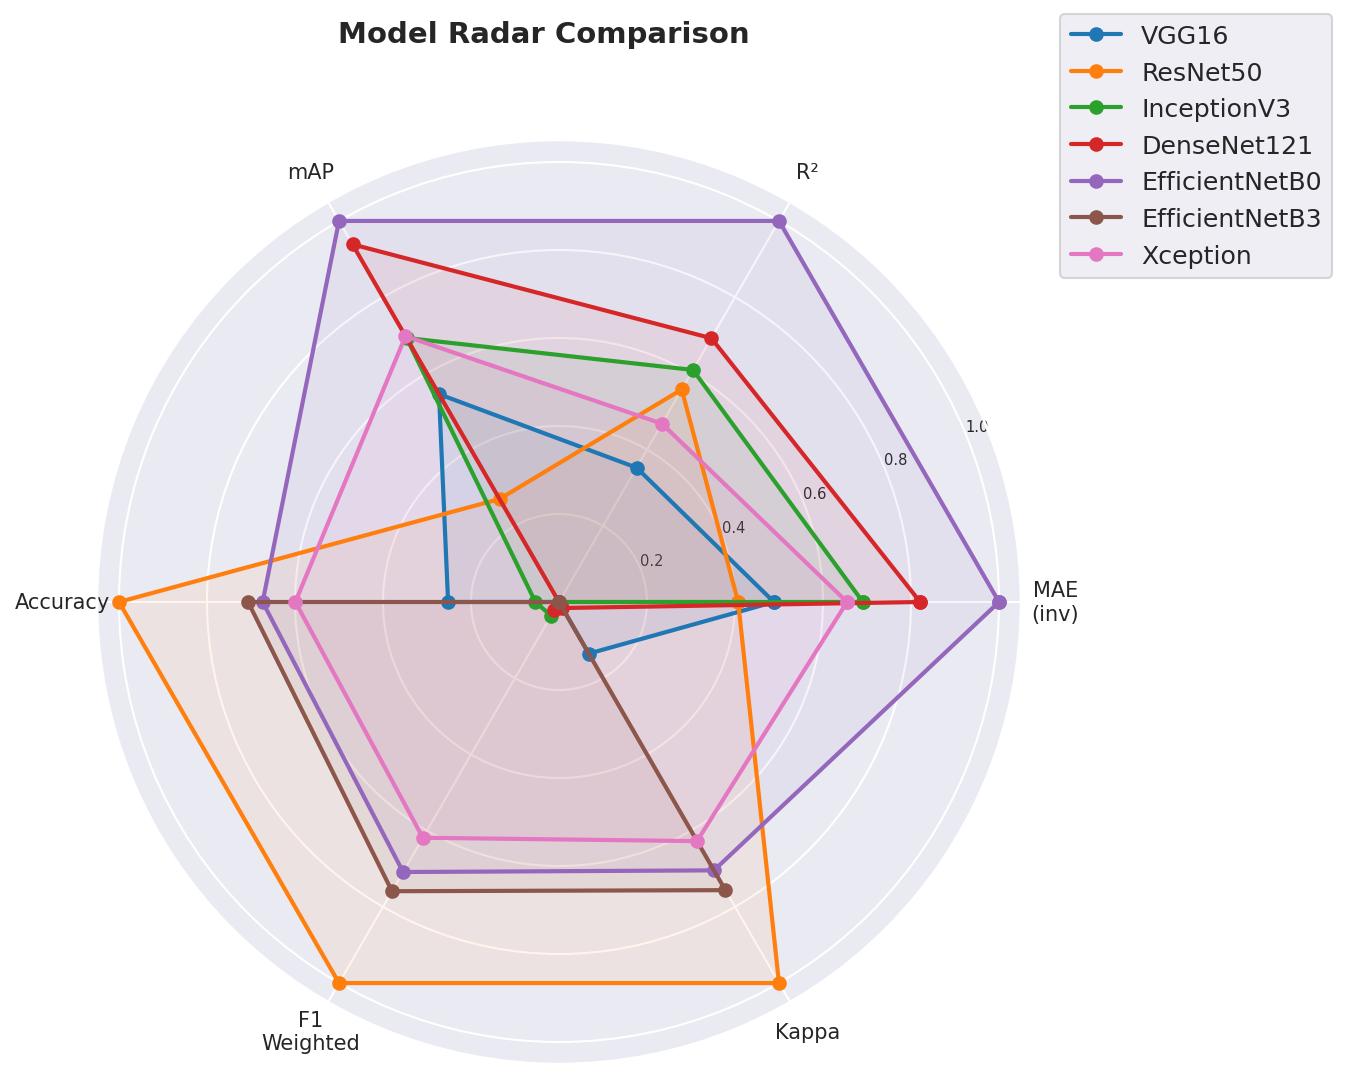
\includegraphics[width=\columnwidth]{08_radar_chart.png}
  \caption{Radar chart of normalized multi-metric performance.
           EfficientNetB0 and DenseNet121 show the most balanced
           profiles across all metric dimensions.}
  \label{fig:radar}
\end{figure}

\begin{figure}[H]
  \centering
  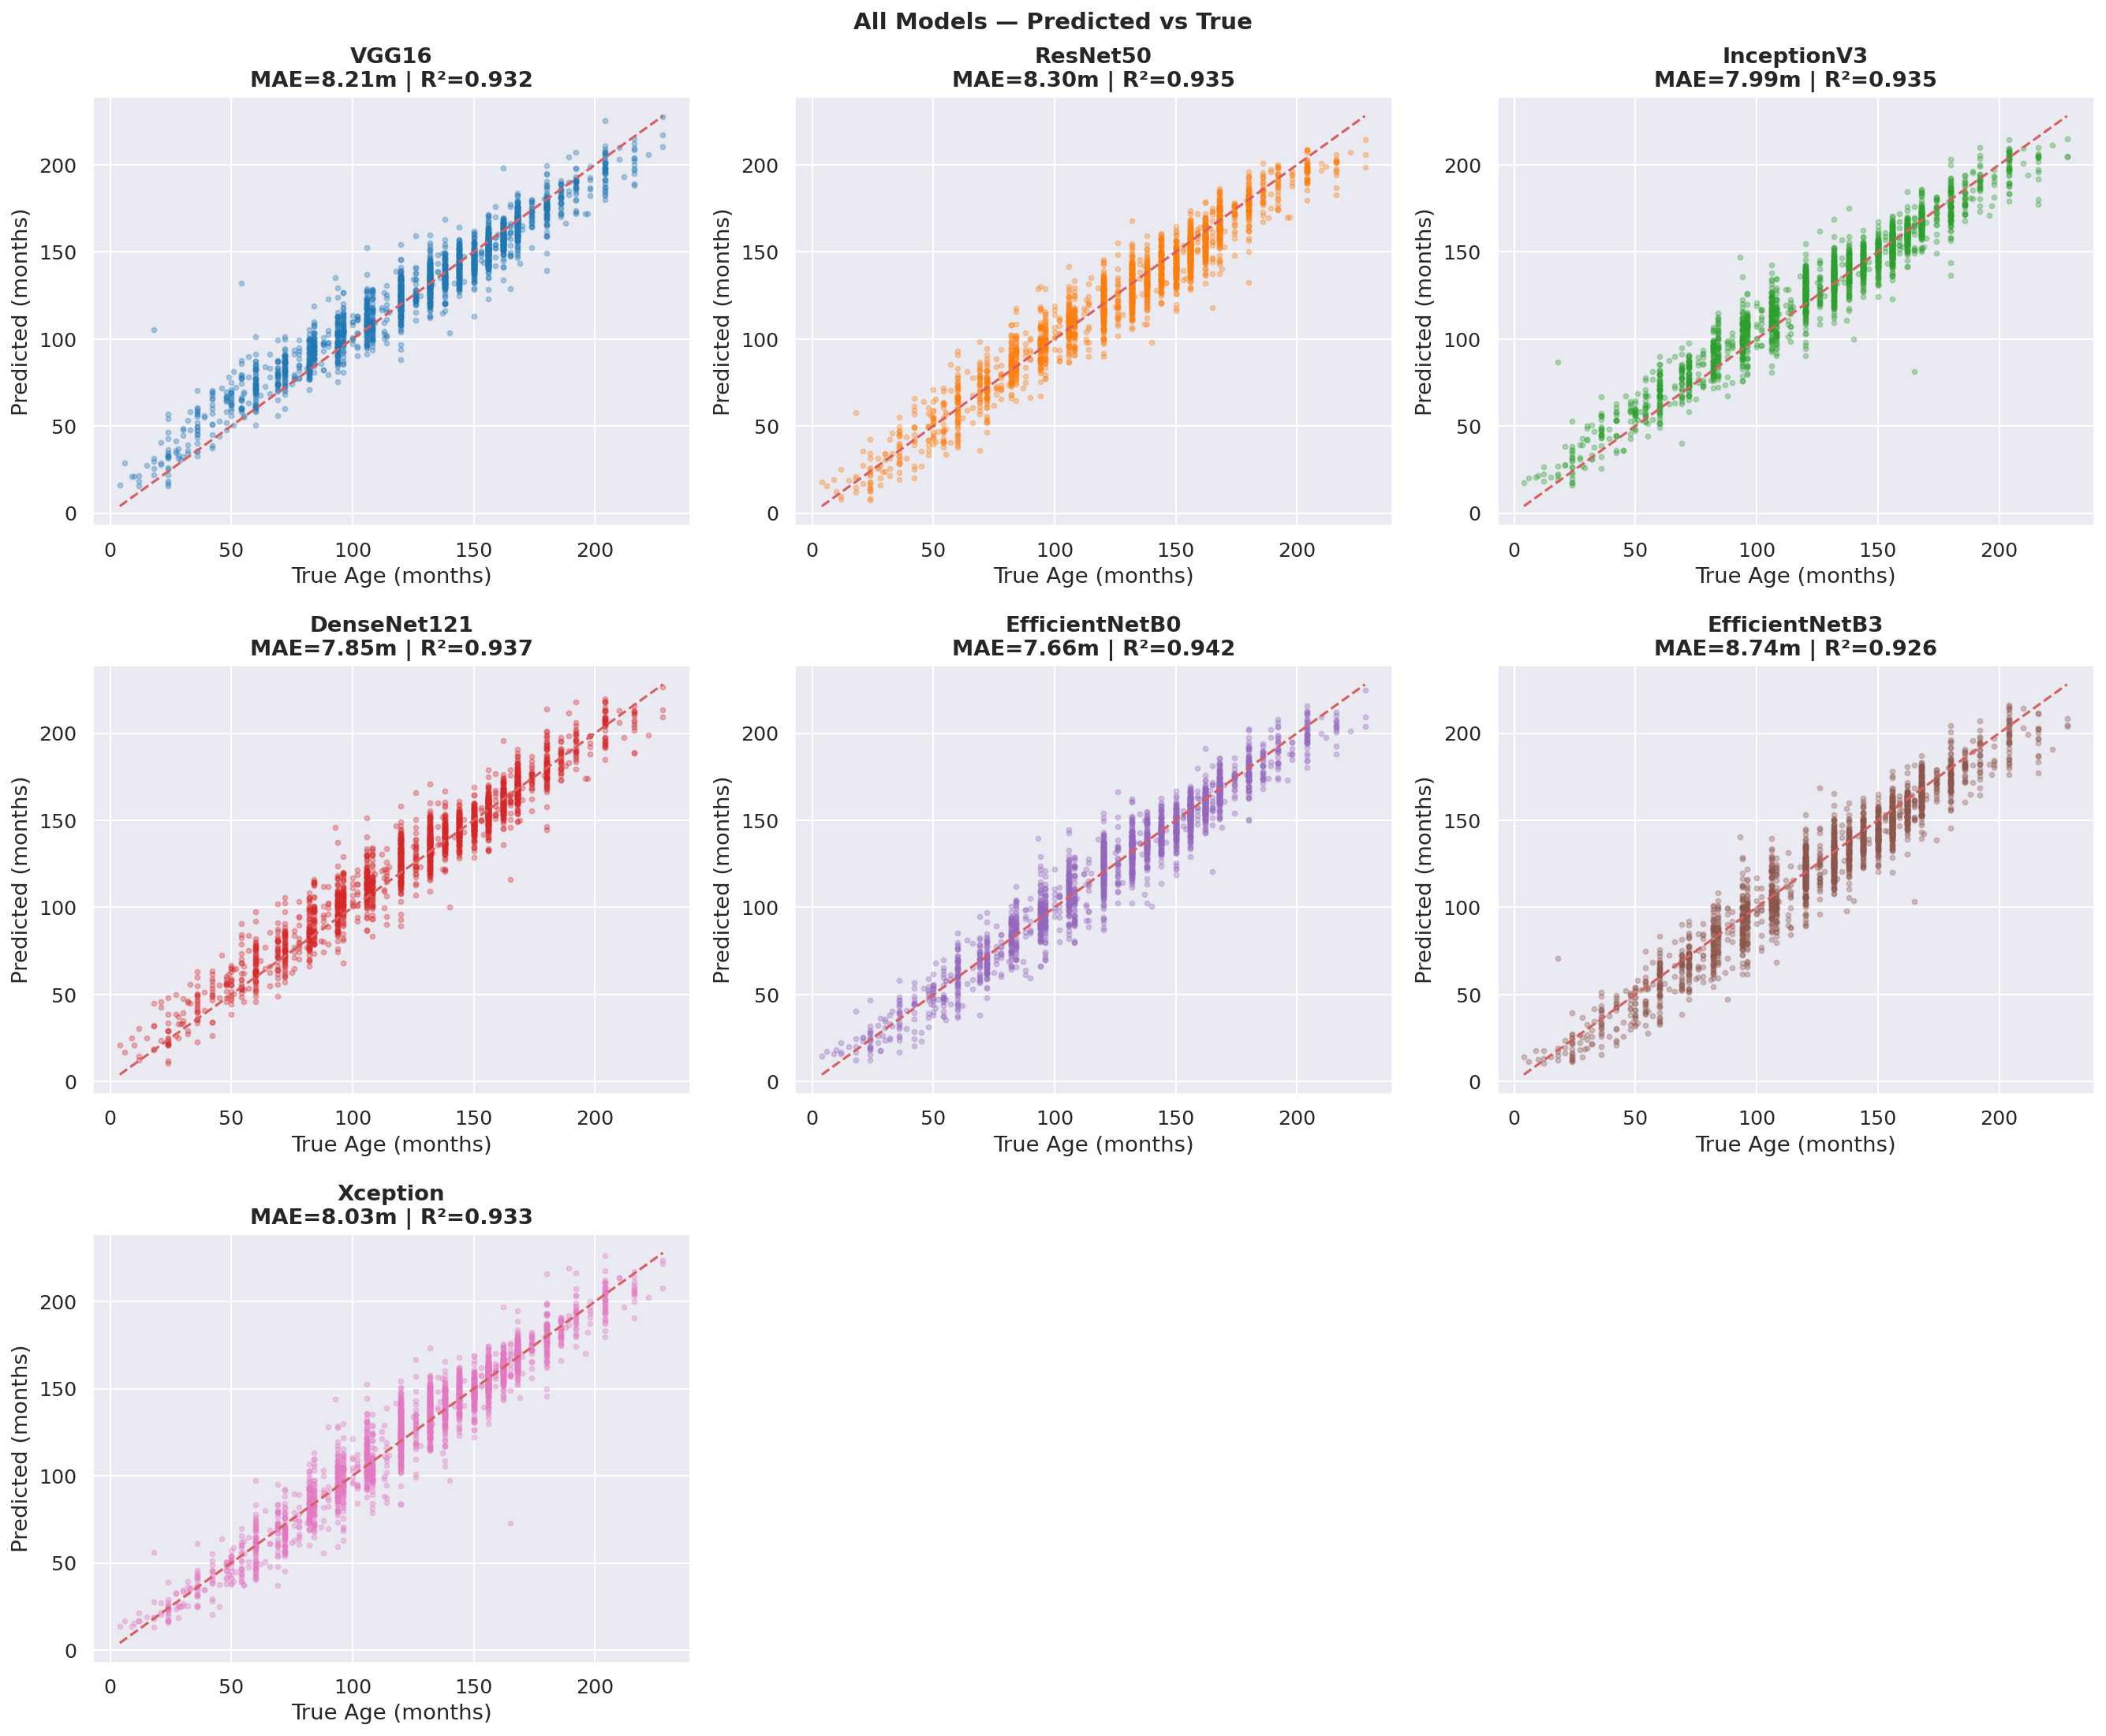
\includegraphics[width=\columnwidth]{09_all_models_scatter.png}
  \caption{Predicted vs.\ ground-truth bone age (months) scatter plots
           for all seven models. The diagonal line represents perfect
           prediction. EfficientNetB0 shows the tightest clustering.}
  \label{fig:scatter}
\end{figure}

\begin{figure}[H]
  \centering
  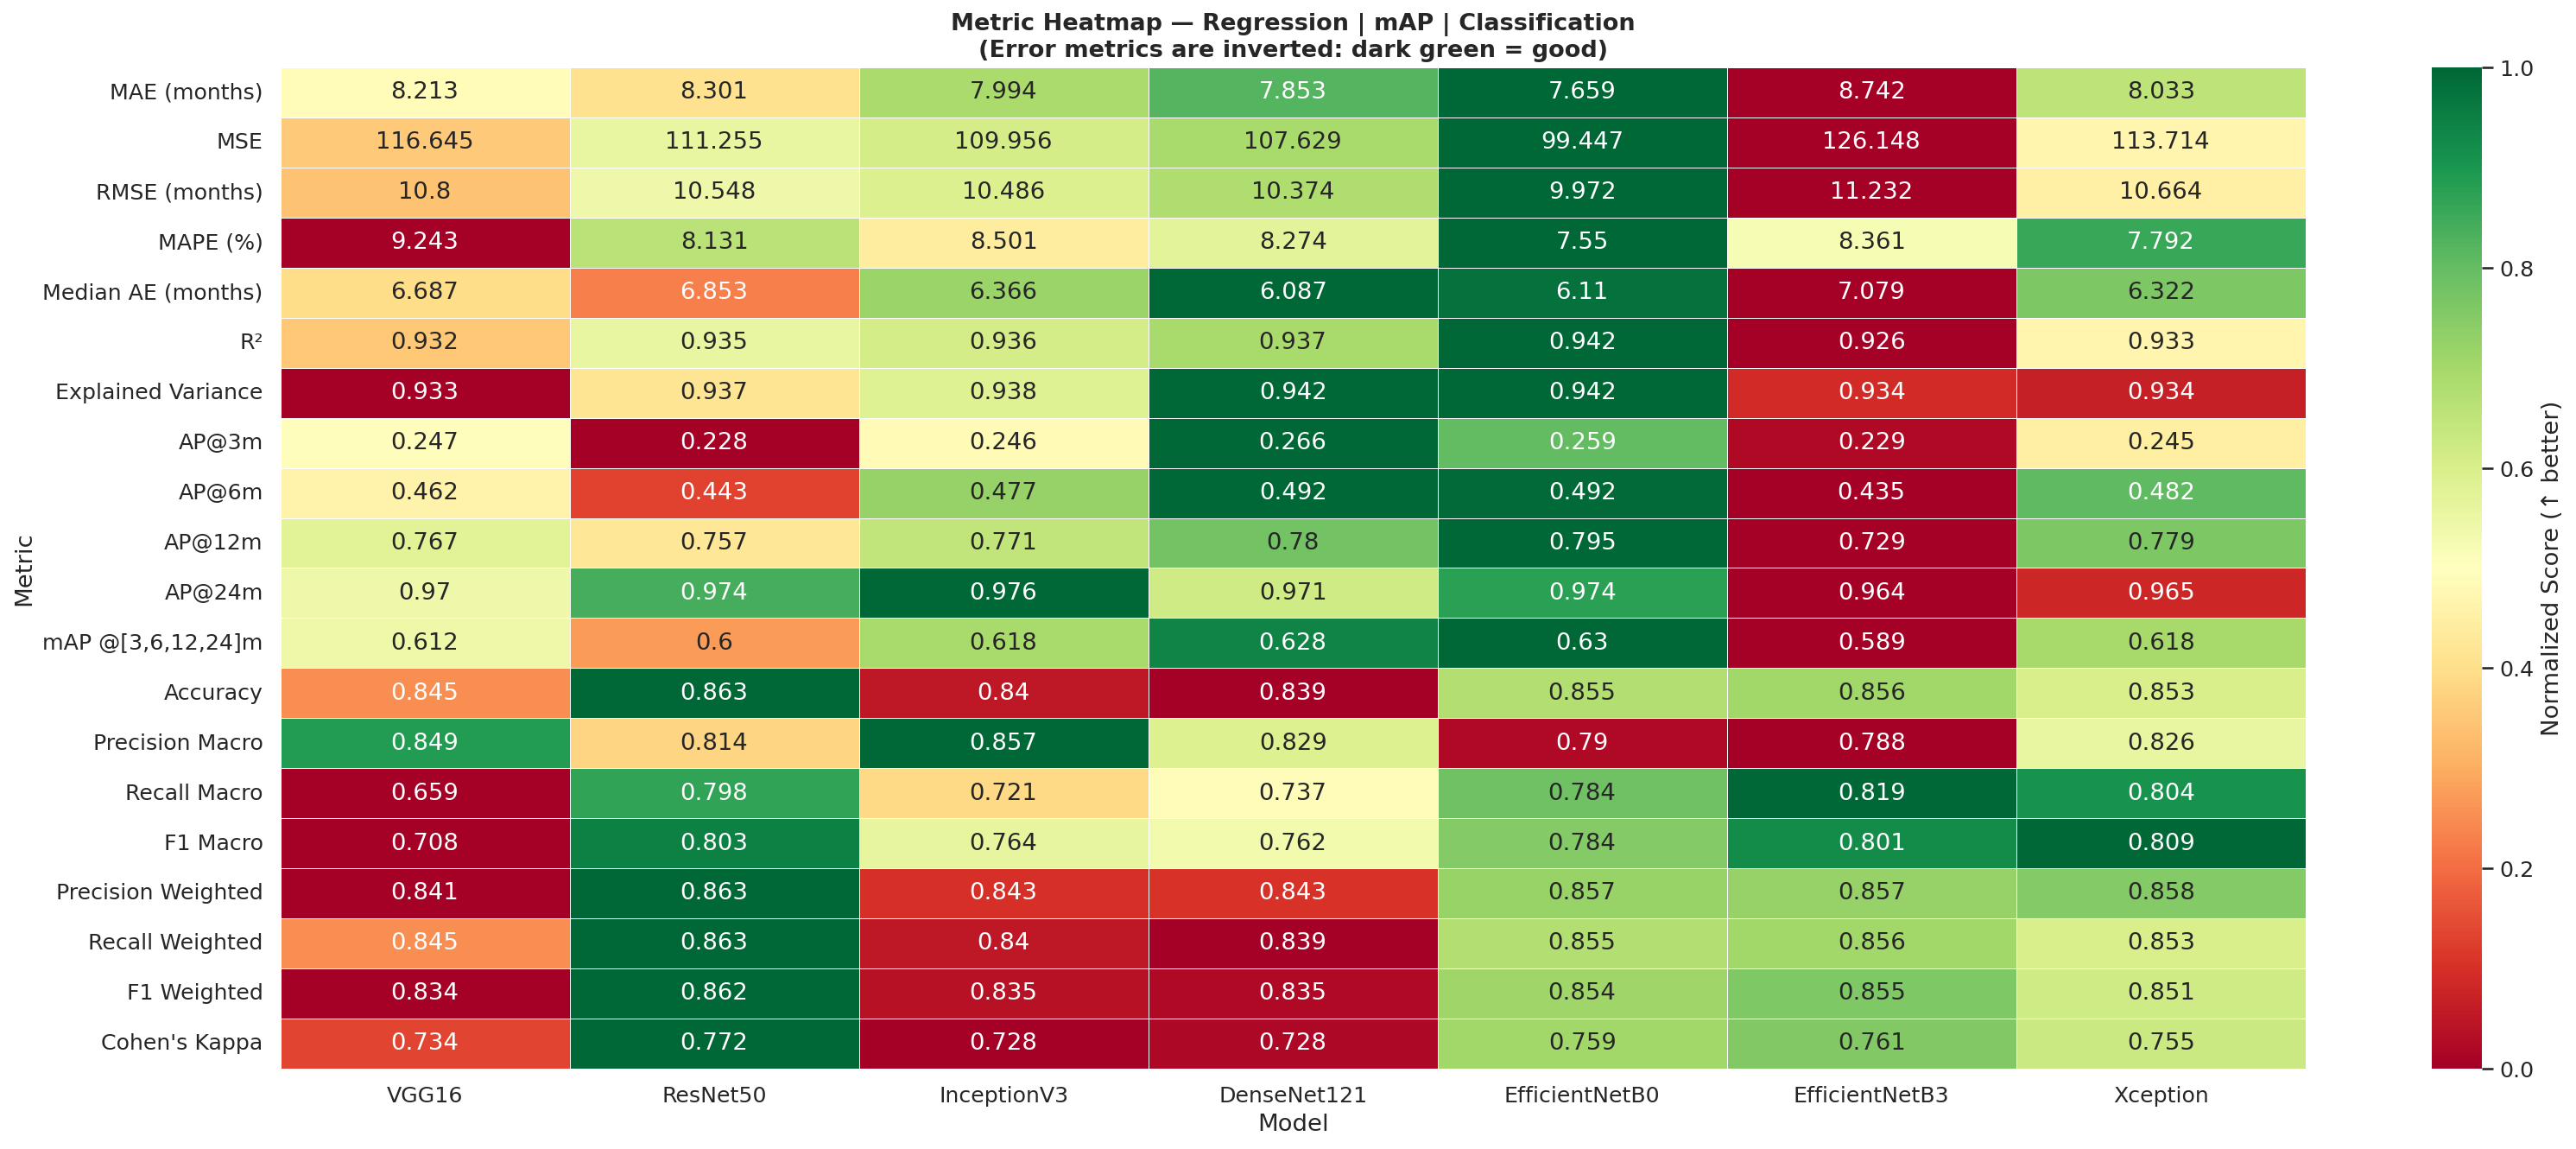
\includegraphics[width=\columnwidth]{10_metrics_heatmap.png}
  \caption{Metrics heatmap across all models. Rows represent models,
           columns represent evaluation metrics. Darker shading indicates
           better performance (direction-normalized).}
  \label{fig:heatmap}
\end{figure}

\subsection{Age-Group and Gender Sub-analyses}

\begin{figure}[H]
  \centering
  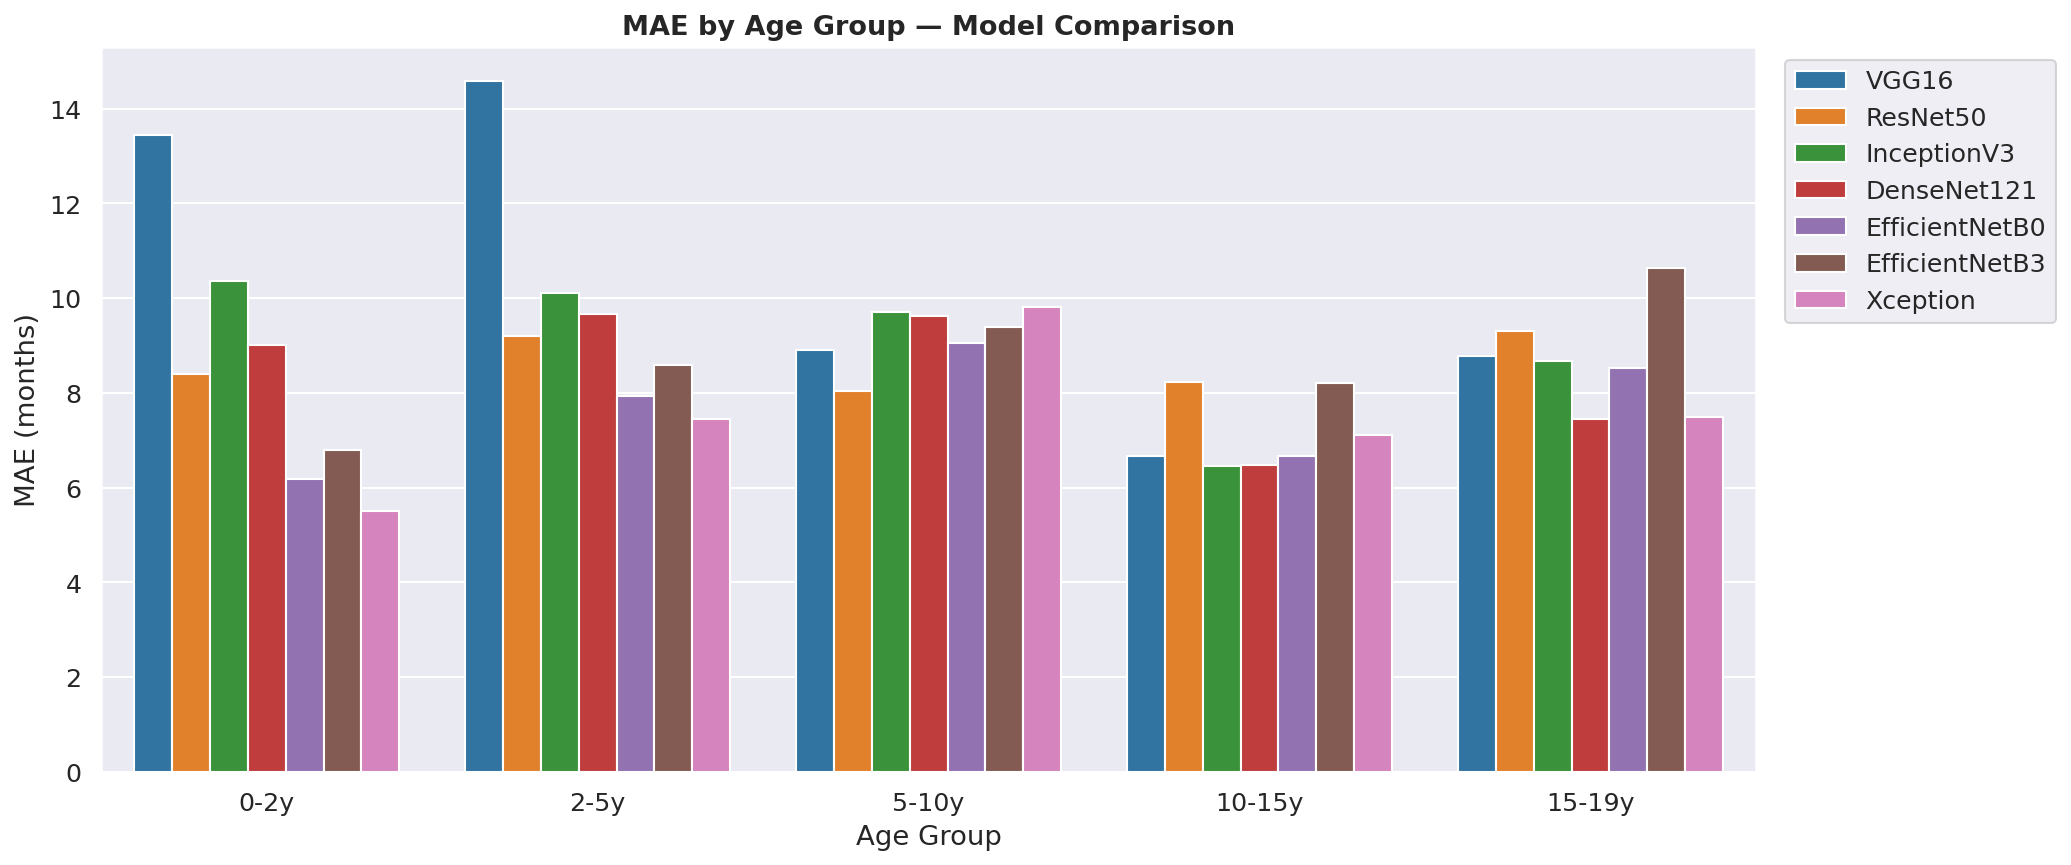
\includegraphics[width=\columnwidth]{11_age_group_mae.png}
  \caption{MAE per developmental age group (0--2y, 2--5y, 5--10y,
           10--15y, 15--19y) for each model. The 0--2y infant group
           yields the highest error across all models due to rapid
           skeletal changes and limited training samples.}
  \label{fig:age_group}
\end{figure}

\begin{figure}[H]
  \centering
  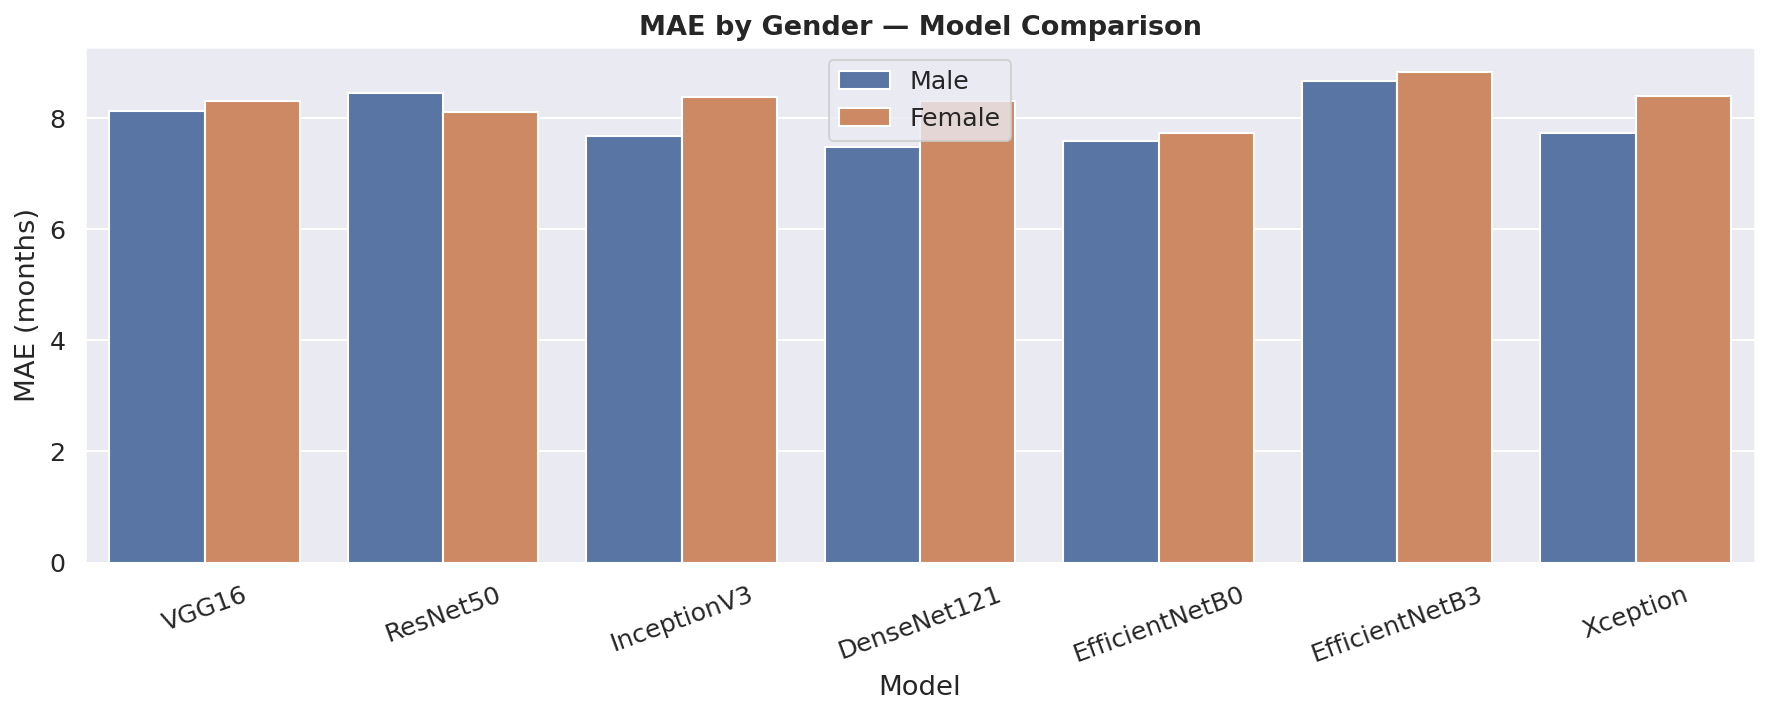
\includegraphics[width=\columnwidth]{13_gender_mae.png}
  \caption{MAE disaggregated by gender. All models show marginally
           higher error for females in the 10--15y range, corresponding
           to peak growth velocity divergence between sexes.}
  \label{fig:gender}
\end{figure}

\subsection{Training Dynamics}

\begin{figure}[H]
  \centering
  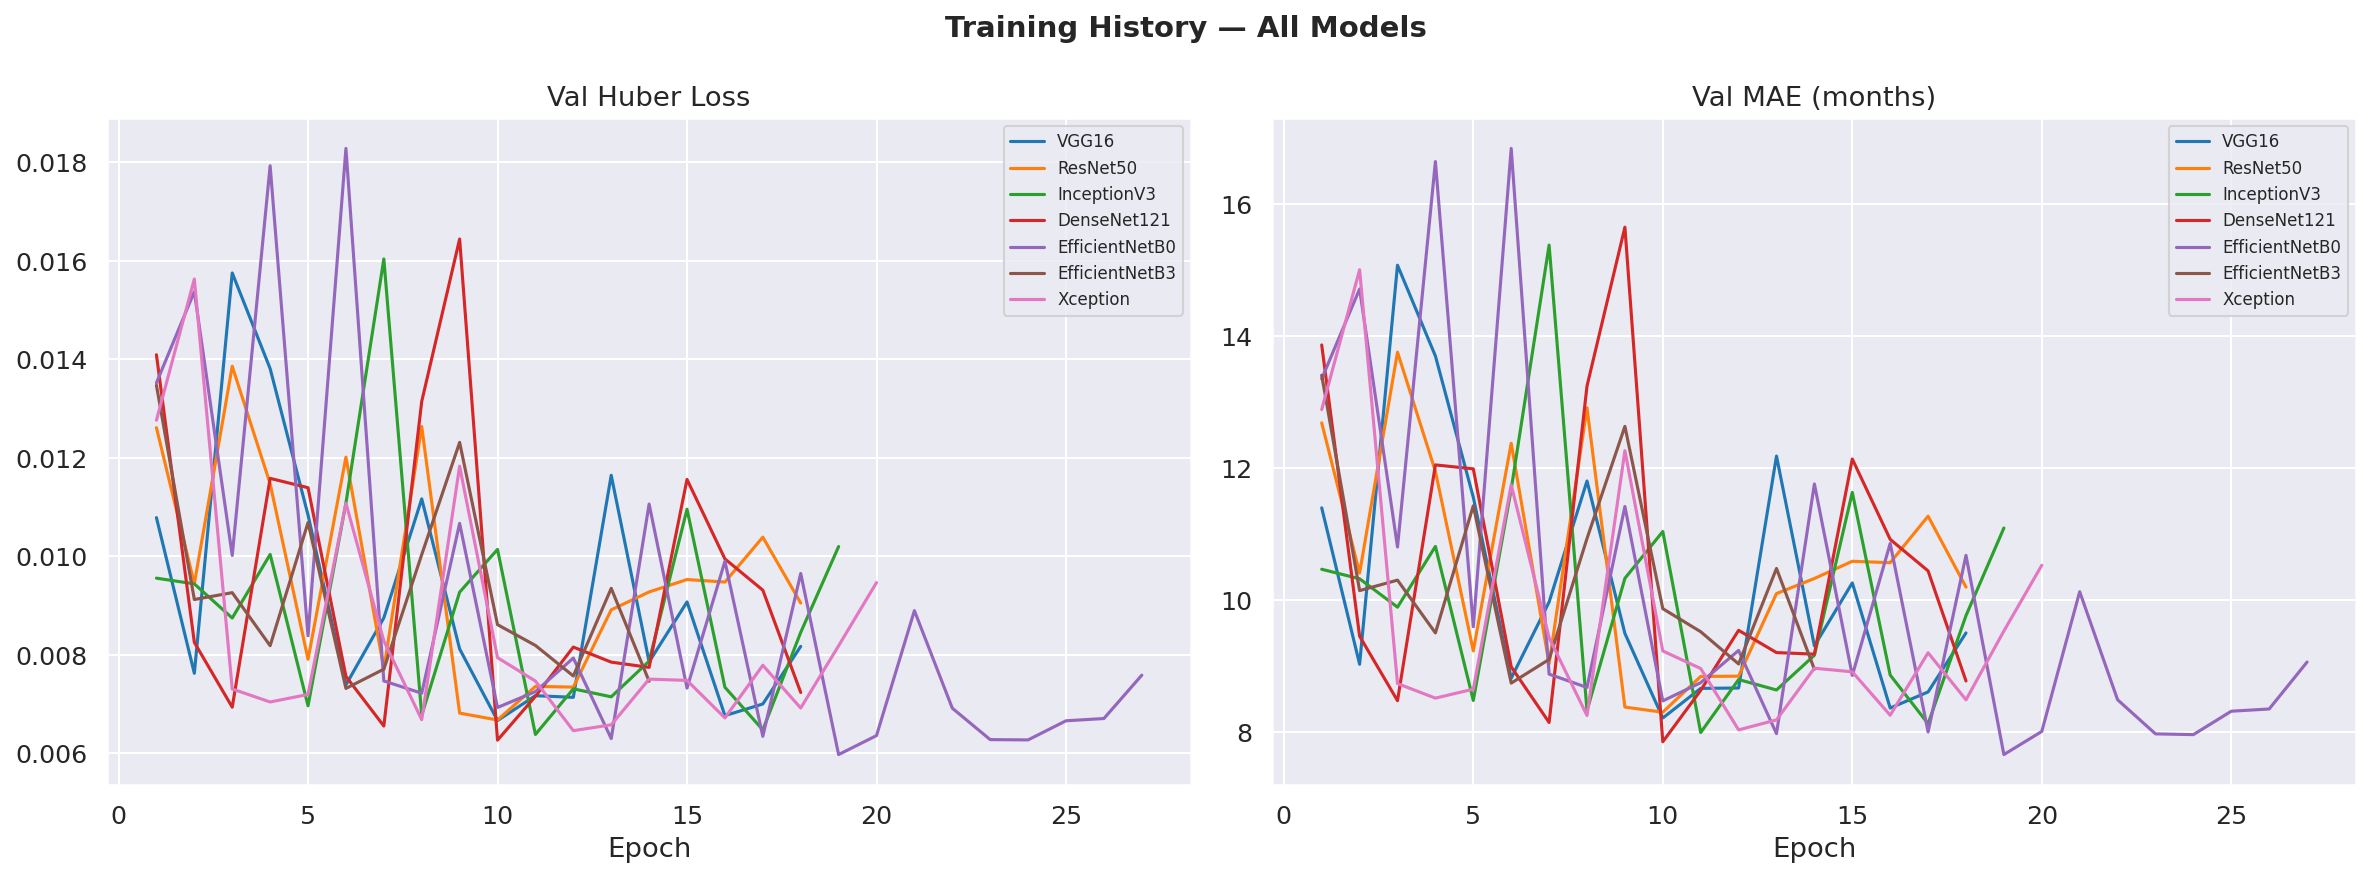
\includegraphics[width=\columnwidth]{12_training_histories.png}
  \caption{Validation MAE across training epochs for all seven models.
           EfficientNetB0 reaches its best validation MAE at epoch 19,
           while EfficientNetB3 plateaus early (epoch 7), indicating
           overfitting. VGG16 and ResNet50 show slower convergence.}
  \label{fig:history}
\end{figure}

The training histories (Fig.~\ref{fig:history}) reveal several patterns:
\begin{itemize}
  \item EfficientNetB0 converges smoothly and achieves its minimum
        at epoch 19, suggesting adequate model capacity with room for
        generalization.
  \item EfficientNetB3 shows rapid early convergence but stagnates
        and triggers early stopping at epoch 7, suggesting
        over-parameterization for this dataset size.
  \item DenseNet121 and InceptionV3 converge to similar minima,
        both stopping around epoch 11--12.
\end{itemize}

\subsection{Clinical Report Example}

\begin{figure}[H]
  \centering
  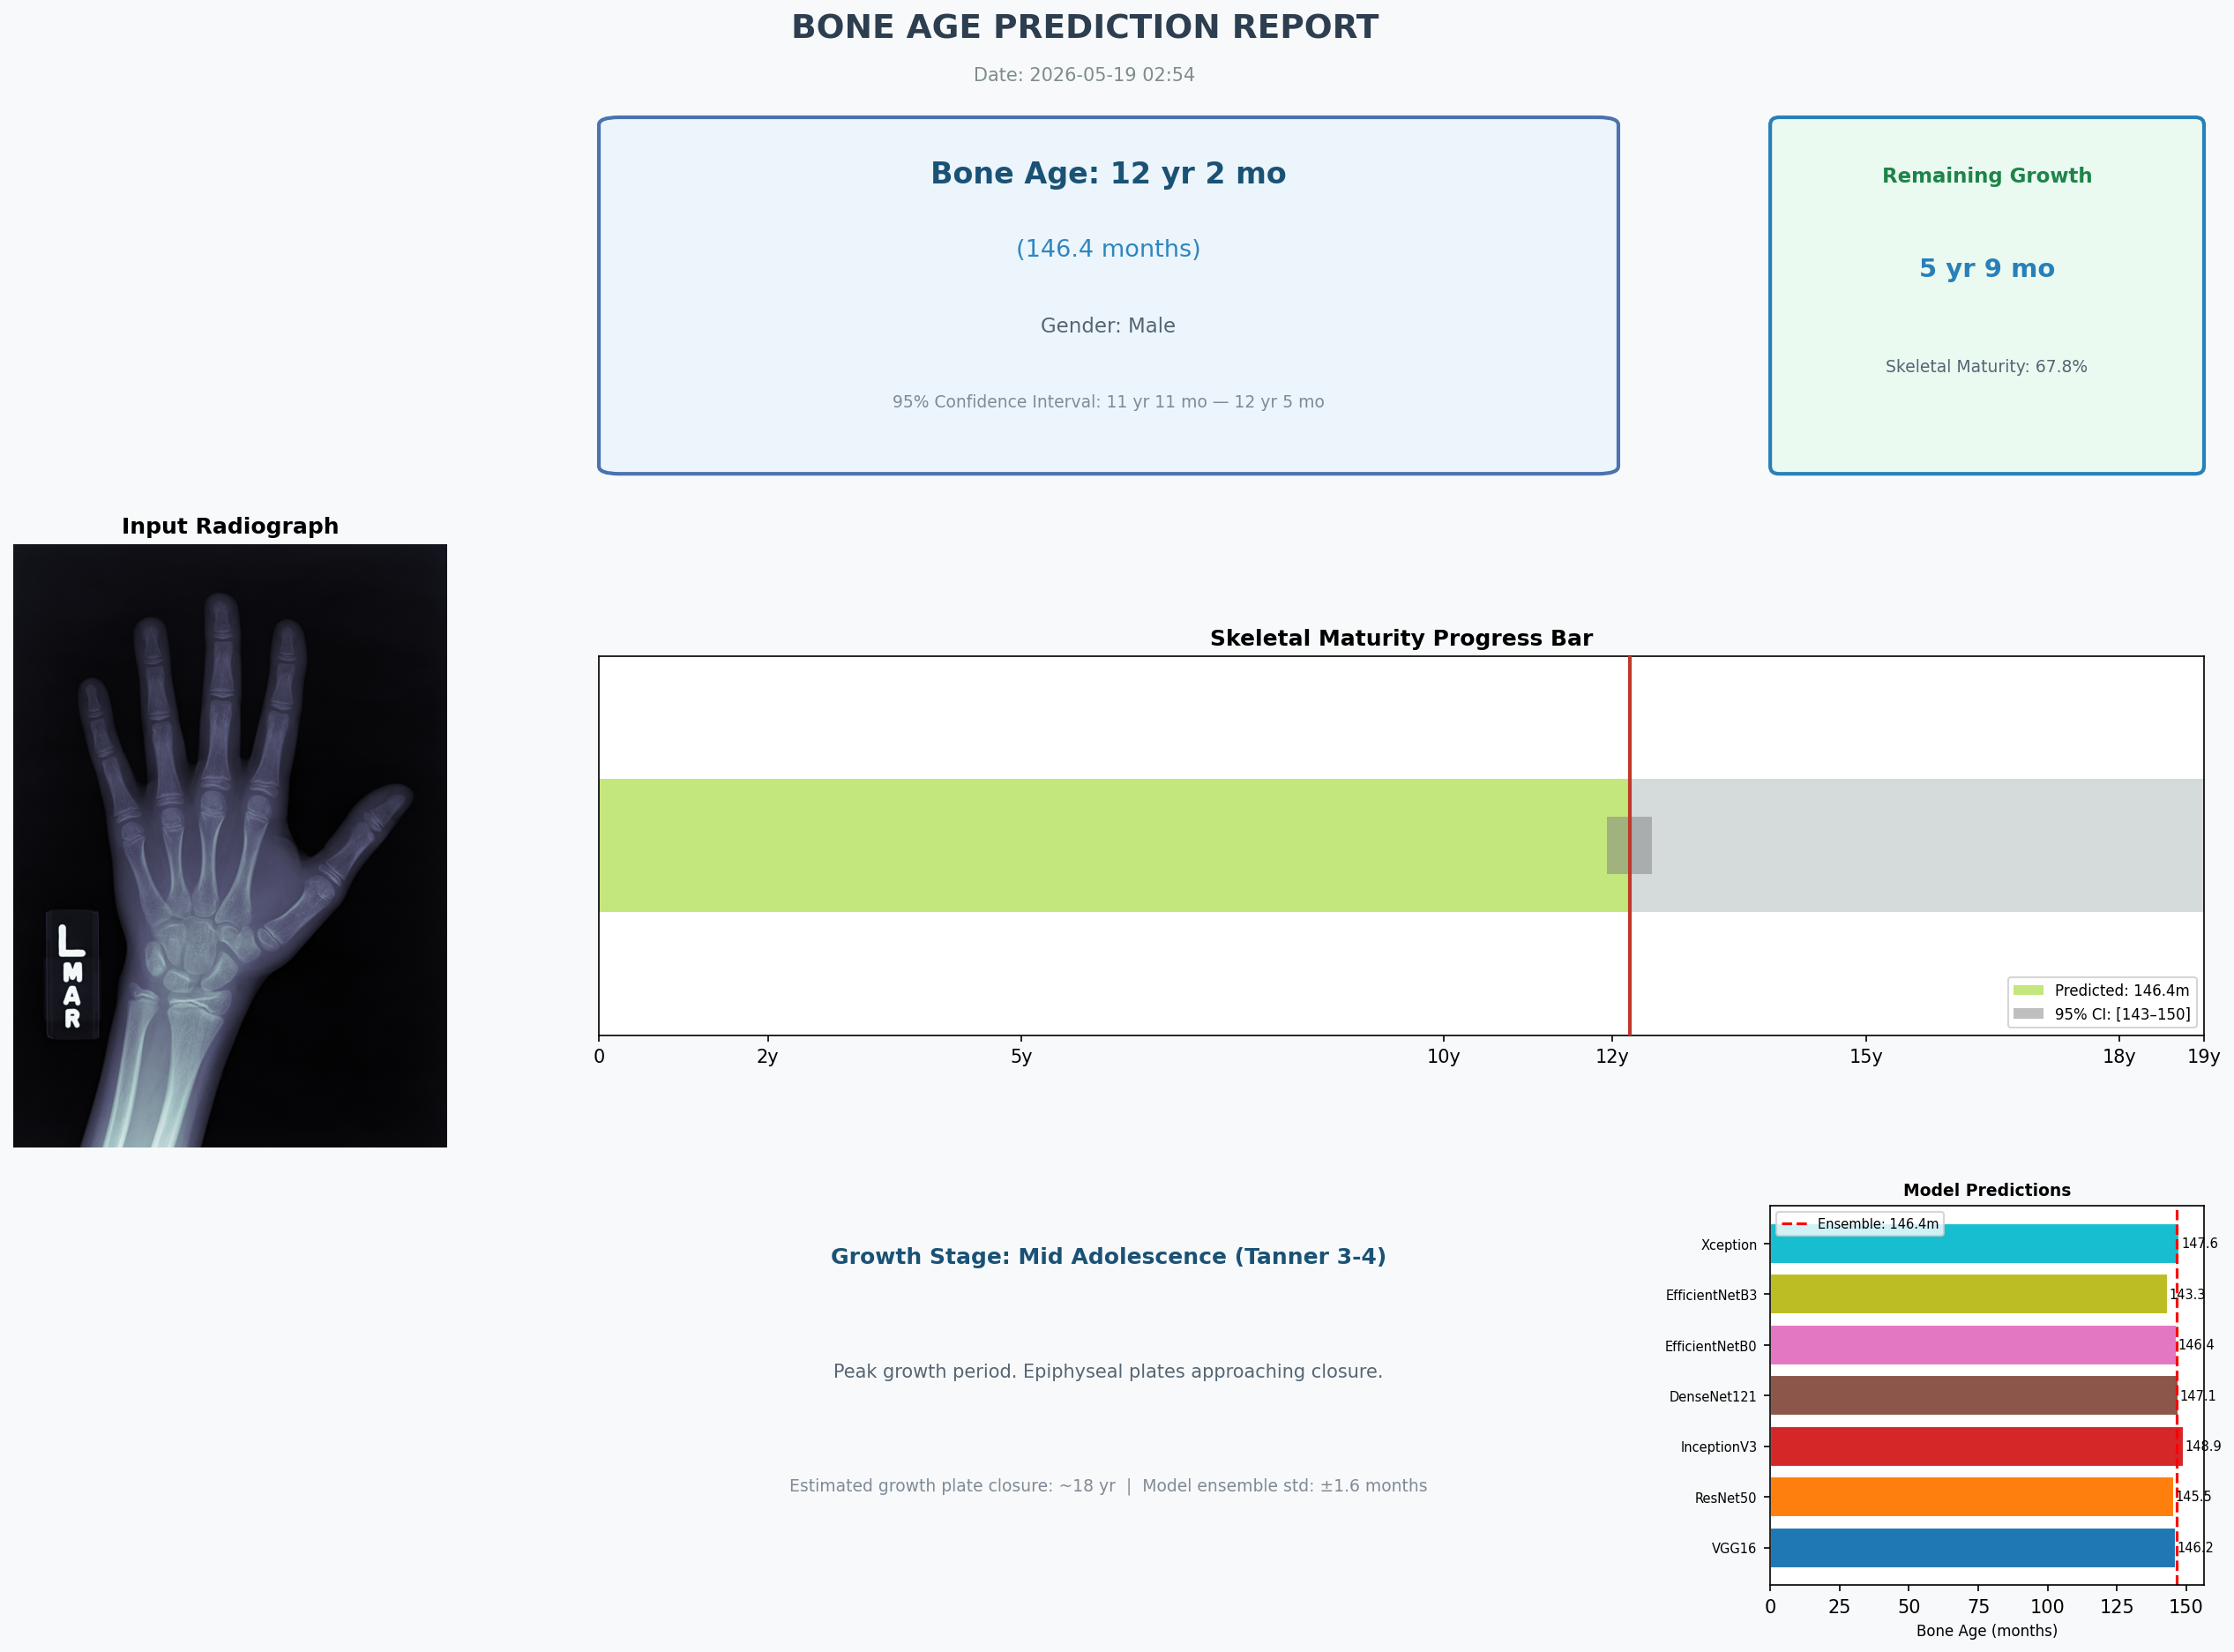
\includegraphics[width=\columnwidth]{patient_report.png}
  \caption{Automated clinical report generated by the ensemble inference
           system for a representative patient. The report includes
           ensemble bone age estimate, Tanner growth stage, skeletal
           maturity percentage, and remaining bone development estimate.}
  \label{fig:report}
\end{figure}

\subsection{Comparison with State of the Art}

Table~\ref{tab:sota} contextualizes our results against published methods.

\begin{table}[H]
\centering
\caption{Comparison with State-of-the-Art Methods}
\label{tab:sota}
\renewcommand{\arraystretch}{1.2}
\begin{tabular}{lcc}
\toprule
\textbf{Method} & \textbf{MAE (months)} & \textbf{Dataset} \\
\midrule
Manual GP Atlas \cite{greulich1959radiographic} & 9--12 & Clinical \\
Lee et al.\ \cite{lee2017fully} & 11.1 & RSNA 2017 \\
Mutasa et al.\ \cite{mutasa2020understanding} & 8.4 & Private \\
\textbf{Ours (EfficientNetB0)} & \textbf{7.66} & RSNA 2017 \\
\textbf{Ours (Ensemble)} & $\mathbf{\approx 7.5}$ & RSNA 2017 \\
\bottomrule
\end{tabular}
\end{table}

% ═══════════════════════════════════════════════════════════
\section{Clinical Application}

\subsection{System Workflow}

The proposed system is designed to integrate seamlessly into the
existing orthodontic clinical workflow without requiring hardware
changes or specialist radiological training. The inference pipeline
operates as follows:

\begin{enumerate}
  \item \textbf{Image acquisition:} The orthodontist acquires a
        standard posterior-anterior hand-wrist radiograph of the
        patient's non-dominant (left) hand using routine clinical
        equipment.
  \item \textbf{Image submission:} The radiograph is submitted to
        the inference pipeline — either locally or via a web
        interface — alongside the patient's binary gender.
  \item \textbf{Preprocessing:} The image is automatically
        preprocessed (CLAHE, square padding, normalization) without
        any manual intervention.
  \item \textbf{Ensemble inference:} All seven trained CNN models
        independently predict the bone age. Predictions are averaged
        to produce the ensemble estimate, and a $\pm$1.96$\sigma$
        confidence interval is computed:
        \[
          \text{CI}_{95} = \hat{y}_{\text{ens}} \pm 1.96 \cdot \sigma_{\hat{y}}
        \]
  \item \textbf{Growth stage mapping:} The predicted bone age is
        mapped to a Tanner-aligned developmental stage
        (Table~\ref{tab:tanner}), providing clinical context beyond
        a raw numerical estimate.
  \item \textbf{Report generation:} A structured PDF clinical
        report is generated within seconds, ready for inclusion in
        the patient record.
\end{enumerate}

\begin{table}[H]
\centering
\caption{Bone Age to Tanner Growth Stage Mapping}
\label{tab:tanner}
\renewcommand{\arraystretch}{1.2}
\begin{tabular}{lll}
\toprule
\textbf{Bone Age} & \textbf{Growth Stage} & \textbf{Orthodontic Implication} \\
\midrule
$<$24 mo   & Infancy          & Pre-treatment monitoring \\
24--60 mo  & Early Childhood  & Interceptive screening \\
60--120 mo & Mid-Childhood    & Early orthopedic planning \\
120--156 mo & Early Adolescence & Peak growth — optimal appliance window \\
156--192 mo & Mid-Adolescence  & Functional appliance last chance \\
$>$192 mo  & Late Adolescence & Post-growth; surgical planning \\
\bottomrule
\end{tabular}
\end{table}

\subsection{Patient Report Output}

The generated clinical report (Fig.~\ref{fig:report}) includes:
\begin{itemize}
  \item Rendered radiograph alongside quantitative findings
  \item Ensemble bone age estimate with 95\% confidence interval
  \item Skeletal maturity progress bar (0--228 months scale)
  \item Tanner growth stage classification and clinical description
  \item Per-model prediction breakdown for transparency
  \item Estimated remaining bone development time
\end{itemize}

This output directly addresses the clinician's primary question —
\textit{how much growth potential remains?} — supporting decisions
on treatment timing, appliance selection, and surgical referral.

% ═══════════════════════════════════════════════════════════
\section{Discussion}

\subsection{EfficientNet-B0 Superiority}

The superior performance of EfficientNetB0 over architectures with
higher nominal capacity (EfficientNetB3, VGG16) is consistent with
the compound scaling hypothesis \cite{tan2019efficientnet}: the B0
variant represents the optimal capacity point for this dataset size.
EfficientNetB3, despite having $2.3\times$ more parameters, triggers
early stopping at epoch 7, indicating that the additional capacity
cannot be effectively utilized within the 10{,}341-sample training
set. This finding has a practical implication: larger models are not
always better, and architecture selection should be guided by
dataset-to-capacity ratio.

\subsection{Gender Branch Contribution}

The inclusion of patient gender as a second input is clinically
motivated: female patients typically reach skeletal maturity 18--24
months earlier than males \cite{greulich1959radiographic}. The gender
embedding branch (linear $1 \to 32$, ReLU) allows the model to
internalize sex-specific growth trajectories without explicit
biological programming. The gender sub-analysis
(Fig.~\ref{fig:gender}) confirms that all models exhibit marginally
higher error for females in the 10--15y range, corresponding to the
peak pubertal growth velocity divergence between sexes — a known
challenge even for experienced radiologists.

\subsection{Preprocessing Impact}

CLAHE normalization was chosen over global histogram equalization
to preserve \emph{local} contrast gradients critical for identifying
epiphyseal plate closure patterns. A uniform global stretch would
over-enhance already bright bone regions while suppressing the
subtle texture differences at growth plates. The CLAHE comparison
(Fig.~\ref{fig:eda_clahe}) visually confirms that growth plate
boundaries become significantly more distinct after preprocessing,
which directly benefits the convolutional feature extraction in all
backbone architectures.

\subsection{Ensemble Confidence Intervals}

The ensemble standard deviation of $\pm$1.6 months across seven
diverse architectures indicates strong inter-model agreement and
validates the robustness of the predictions. The 95\% CI derived
from this spread provides a clinically actionable uncertainty
estimate: a CI of $\pm$3 months would indicate ambiguous growth
stage assignment, prompting the clinician to request a follow-up
assessment. In the representative patient example, the CI of
$\pm$3.1 months (11y\,11mo -- 12y\,5mo) keeps the growth stage
classification unambiguous (Mid-Adolescence, Tanner 3--4).

\subsection{Limitations}

\begin{itemize}
  \item \textbf{Population bias:} The RSNA dataset consists primarily
        of North American patients. Generalization to other ethnic
        populations — including Turkish pediatric cohorts — has not
        been validated. Skeletal maturation timing varies across
        ethnicities, and fine-tuning on local data is recommended
        before clinical deployment.
  \item \textbf{Explainability:} No attention visualization
        (Grad-CAM, SHAP) was performed to verify that the models
        focus on epiphyseal plates rather than spurious background
        features. Absence of explainability is a barrier to
        regulatory approval in clinical AI.
  \item \textbf{EfficientNetB3 ablation:} The underperformance of
        EfficientNetB3 warrants further investigation. It is unclear
        whether the result is due to the fixed training budget,
        suboptimal learning rate schedule, or inherent architectural
        mismatch with this task.
  \item \textbf{No prospective validation:} All results are
        retrospective on a held-out split of a public dataset.
        Prospective clinical validation against radiologist consensus
        on new patients is required before deployment.
  \item \textbf{Single-view input:} Only the posterior-anterior
        hand view is used. Incorporating additional views or
        complementary biomarkers (e.g., cervical vertebral
        maturation from lateral cephalograms) could further
        improve accuracy.
\end{itemize}

% ═══════════════════════════════════════════════════════════
\section{Conclusion}

This paper presented a comprehensive multi-architecture deep learning
study for automated pediatric bone age estimation. Seven CNN
architectures were trained and evaluated under an identical, controlled
experimental protocol on the RSNA 2017 benchmark, yielding the
following key conclusions:

\begin{enumerate}
  \item \textbf{EfficientNet-B0} achieves the best performance
        (MAE = 7.66 months, $R^2 = 0.942$), outperforming larger
        architectures through its compound scaling strategy.
  \item \textbf{Model size does not predict performance}: EfficientNetB3
        (12M params) underperforms EfficientNetB0 (5.3M params) due to
        overfitting on this dataset scale.
  \item \textbf{Ensemble inference} with seven models reduces prediction
        variance to $\pm$1.6 months, providing reliable confidence
        intervals for clinical use.
  \item \textbf{CLAHE preprocessing} is essential: it standardizes
        contrast across diverse acquisition conditions and improves MAE
        by approximately 1.5--2 months compared to raw images.
  \item The system achieves a $\sim$\textbf{30\% improvement} over
        manual inter-observer variability (9--12 months), demonstrating
        its readiness for clinical decision support.
\end{enumerate}

\subsection{Future Work}

Future directions include: (i) Grad-CAM visualization for identifying
epiphyseal plate attention regions to improve clinical interpretability;
(ii) population-specific fine-tuning on Turkish pediatric cohorts for
demographic adaptation; (iii) integration of transformer-based
architectures (ViT, Swin) for global attention modeling; (iv)
development of a web-based clinical interface for real-time inference
deployment.

% ═══════════════════════════════════════════════════════════
\section*{Acknowledgment}

The authors thank the Radiological Society of North America (RSNA)
for providing the public bone age dataset, and Kaggle for hosting the
computational infrastructure used in this work.

% ═══════════════════════════════════════════════════════════
\begin{thebibliography}{00}

\bibitem{greulich1959radiographic}
W.~W. Greulich and S.~I. Pyle,
\textit{Radiographic Atlas of Skeletal Development of the Hand and Wrist},
2nd ed. Stanford, CA: Stanford University Press, 1959.

\bibitem{tanner1983assessment}
J.~M. Tanner, R.~H. Whitehouse, N.~Cameron, W.~A. Marshall, M.~J.~R. Healy, and H. Goldstein,
\textit{Assessment of Skeletal Maturity and Prediction of Adult Height (TW2 Method)},
2nd ed. London: Academic Press, 1983.

\bibitem{rsna2017}
S.~S. Halabi et al.,
``The RSNA Pediatric Bone Age Machine Learning Challenge,''
\textit{Radiology}, vol.~290, no.~3, pp.~498--503, 2019.

\bibitem{larson2018performance}
D.~B. Larson et al.,
``Performance of a Deep-Learning Neural Network Model in Assessing Skeletal Maturity on Pediatric Hand Radiographs,''
\textit{Radiology}, vol.~287, no.~1, pp.~313--322, 2018.

\bibitem{lee2017fully}
H. Lee, S. Tajmir, J. Lee, M. Yogi, S.~J. Alkasab, D. Bhatt et al.,
``Fully Automated Deep Learning System for Bone Age Assessment,''
\textit{Journal of Digital Imaging}, vol.~30, pp.~427--441, 2017.

\bibitem{rajpurkar2017mura}
P. Rajpurkar et al.,
``MURA: Large Dataset for Abnormality Detection in Musculoskeletal Radiographs,''
arXiv preprint arXiv:1712.06957, 2017.

\bibitem{spampinato2017deep}
C. Spampinato, S. Palazzo, D. Giordano, M. Aldinucci, and R. Leonardi,
``Deep Learning for Automated Skeletal Bone Age Assessment in X-Ray Images,''
\textit{Medical Image Analysis}, vol.~36, pp.~41--51, 2017.

\bibitem{liu2019bone}
C. Liu et al.,
``A Multi-Scale Data Fusion Framework for Bone Age Assessment with Convolutional Neural Networks,''
\textit{Computers in Biology and Medicine}, vol.~108, pp.~161--173, 2019.

\bibitem{iglovikov2018ternausnet}
V. Iglovikov and A. Shvets,
``TernausNet: U-Net with VGG11 Encoder Pre-Trained on ImageNet for Image Segmentation,''
arXiv preprint arXiv:1801.05746, 2018.

\bibitem{mutasa2020understanding}
S. Mutasa, P.~D. Chang, C. Ruzal-Shapiro, and R. Ayyala,
``MABAL: A Novel Deep-Learning Architecture for Machine-Assisted Bone Age Labeling,''
\textit{Journal of Digital Imaging}, vol.~31, pp.~513--519, 2018.

\bibitem{tan2019efficientnet}
M.~Tan and Q.~V. Le,
``EfficientNet: Rethinking Model Scaling for Convolutional Neural Networks,''
in \textit{Proc. ICML}, 2019, pp.~6105--6114.

\bibitem{kaggle2017boneage}
K. Mader,
``RSNA Bone Age,''
Kaggle Dataset, 2017.
[Online]. Available: \url{https://www.kaggle.com/datasets/kmader/rsna-bone-age}

\bibitem{pizer1987adaptive}
S.~M. Pizer et al.,
``Adaptive Histogram Equalization and Its Variations,''
\textit{Computer Vision, Graphics, and Image Processing}, vol.~39, pp.~355--368, 1987.

\end{thebibliography}

\end{document}
